% Created 2012-06-14 Thu 12:35
\documentclass[11pt]{article}
\usepackage[utf8]{inputenc}
\usepackage[T1]{fontenc}
\usepackage{fixltx2e}
\usepackage{graphicx}
\usepackage{longtable}
\usepackage{float}
\usepackage{wrapfig}
\usepackage{soul}
\usepackage{textcomp}
\usepackage{marvosym}
\usepackage{wasysym}
\usepackage{latexsym}
\usepackage{amssymb}
\usepackage{hyperref}
\tolerance=1000
\usepackage[T1]{fontenc}
\usepackage[spanish]{babel}
\usepackage[margin=2.5cm,includefoot]{geometry}
\usepackage{graphicx}
\usepackage{pict2e}
\usepackage{amsmath}
\usepackage{chngcntr}
\usepackage{hyperref}
\hypersetup{
colorlinks,%
citecolor=green,%
filecolor=black,%
linkcolor=blue,%
urlcolor=blue
}
\providecommand{\alert}[1]{\textbf{#1}}

\title{Entrenamiento por refuerzo de redes neuronales mediante algoritmos gen\'eticos}
\author{Jorge Tim\'on Morillo-Velarde \\textbackslash{} href\{mailto:jtimonmv@gmail.com\}{jtimonmv@gmail.com\}}
\date{\today}
\hypersetup{
  pdfkeywords={Redes neuronales, algoritmos gen\'eticos, redes neuronales evolutivas, aprendizaje por refuerzo, CUDA, entornos artificiales, juegos multi-agente.},
  pdfsubject={},
  pdfcreator={Emacs Org-mode version 7.8.09}}

\begin{document}





\setcounter{secnumdepth}{5}
\counterwithin{figure}{section}
\setcounter{tocdepth}{5}

\newcommand{\mail}[1][timon.elviejo@gmail.com]{%
e-mail: \href{mailto:#1} {#1}
}

\newcommand{\definicion}[1]{%
    \textbullet \bfseries{ #1 :}
}

\newenvironment{listaDefiniciones}%
%ordenes al inicio
{
\begin{list}{}%
     {  \setlength{\itemsep}{0.5ex}
    \setlength{\parsep}{0.5ex}
    \setlength{\partopsep}{0.5ex}
    \setlength{\topsep}{\dimexpr 2\itemsep}
    \setlength{\listparindent}{\dimexpr \parindent}
    \renewcommand*{\makelabel}[1]{\definicion{##1}}
    }
}
%ordenes al final
{
\end{list}
}%



\begin{titlepage}

\title{Entrenamiento por refuerzo de redes neuronales mediante algoritmos gen\'eticos}
\newline
\newline
\newline

\author{
\\ Autor:\\
\\ Jorge Tim\'on Morillo-Velarde \\ \mail
\\ \\ \\ \\
\\ Tutores del proyecto:\\ 
\\ Rosa M. P\'erez Utrero \\ \mail[rosapere@unex.es]
\\ 
\\ Juan A. G\'omez Pulido \\ \mail[jangomez@unex.es]
\\ \\ \\ \\
}

\date{\today}

\maketitle
\newpage

\begin{abstract}

En este trabajo se estudia un m\'etodo alternativo para el entrenamiento de redes neuronales con conexi\'on hacia delante. Se utiliza un algoritmo gen\'etico para ajustar los pesos de la red neuronal. Se eval\'ua el uso de diferentes tipos de neuronas (con salida real o binaria) para comparar sus rendimientos utilizando diferentes implementaciones paralelas (para el coprocesador XMM y para la arquitectura CUDA). Se prueban variaciones de los operadores gen\'eticos y se mide su efectividad en el entrenamiento. Se enfrenta el algoritmo a diferentes tipos de problemas de aprendizaje por refuerzo y se medita sobre la idoneidad del mismo para cada problema.
\\

\textbf{Palabras clave:} Redes neuronales, algoritmos gen\'eticos, redes neuronales evolutivas, aprendizaje por refuerzo, CUDA, entornos artificiales, juegos multi-agente.

\end{abstract}

\newpage

\tableofcontents

\newpage

\section{Introducci\'on}
\label{sec-1}

  \label{intro}

 El aprendizaje autom\'atico es una rama de la inteligencia artificial que trata de construir sistemas inform\'aticos que optimicen un criterio de rendimiento utilizando datos o experiencia previa. Dentro del aprendizaje autom\'atico, las t\'ecnicas se clasifican en base a su entrenamiento como supervisado o no supervisado. En el primero, al sistema se le suministran ejemplos de entradas con sus correspondientes salidas deseadas. En el entrenamiento no supervisado, no se tienen a priori ejemplos de c\'omo deber\'ia comportarse el sistema. El aprendizaje por refuerzo es un caso especial de aprendizaje supervisado en que la salida deseada exacta es desconocida. Se basa s\'olo en informaci\'on sobre si la salida actual es correcta o no. Al agente que se quiere que aprenda se le provee informaci\'on sobre lo bien o lo mal que est\'a actuando. Esta se\~nal de recompensa puede serle indicada bien cada vez que el agente act\'ua, bien al final de una prueba completa durante la que realiza varias acciones.

 Los algoritmos que tienen su origen en la observaci\'on de la naturaleza se denominan bio-inspirados. Entre ellos se encuentran las redes neuronales y los algoritmos gen\'eticos. 

 Las redes neuronales son modelos que intentan reproducir el comportamiento del cerebro humano [Hilera y Mart\'inez, 1995]. Una red neuronal consiste en un conjunto de elementos de procesamiento, llamados neuronas, los cuales se conectan entre s\'i [Koehn, 1994]. Las conexiones entre las neuronas tienen pesos asociados cuyos valores determinar\'an el comportamiento de la red. Existen algoritmos para determinar el valor de los pesos de una red mediante un entrenamiento supervisado, cabe destacar el de retro-propagaci\'on del error.

 Los algoritmos evolutivos, dentro de los cuales los algoritmos gen\'eticos son los m\'as conocidos, son una familia de modelos computacionales inspirados en la evoluci\'on y la supervivencia del m\'as apto [B\"ach, et. al., 1991; \"Omer, 1995; Whitley, 2001]. Se utilizan fundamentalmente en la resoluci\'on de problemas de b\'usqueda y de optimizaci\'on [Holland, 1975]. Buscan una soluci\'on del problema reproduciendo gen\'eticamente una poblaci\'on de individuos a lo largo de una serie de generaciones [Koza, 1997]. El aprendizaje es formulado como un problema de optimizaci\'on, en el que cada individuo de la poblaci\'on es una posible soluci\'on.

 Dada una topolog\'ia de red fija, el entrenamiento de una red neuronal puede ser visto como un proceso de optimizaci\'on cuyo objetivo es encontrar un conjunto de pesos que minimice el error que produce la red sobre el conjunto de ejemplos en el entrenamiento supervisado, o que maximice la recompensa en el aprendizaje por refuerzo.

 En nuestro caso, el agente utilizar\'a una red neuronal para decidir sus acciones (salida de la red) a partir de los datos que pueda recoger de su entorno (entrada a la red). Se utiliza un algoritmo gen\'etico para decidir los pesos adecuados para la red, utilizando una poblaci\'on de agentes con redes diferentes. Se utiliza la recompensa acumulada por el individuo en una o varias pruebas para medir su adaptaci\'on al medio. Se utilizan estas medidas y la poblaci\'on actual para construir la siguiente generaci\'on. Cuando alg\'un individuo demuestra estar lo suficientemente adaptado al medio para cumplir con las expectativas del entrenamiento (o cuando se supera un l\'imite prefijado de iteraciones), \'este finaliza.

 En todo este proceso, El algoritmo que m\'as se ejecuta es el que calcula la salida de la red a partir de la entrada. Este algoritmo se puede llamar varias veces por cada prueba. Adem\'as, las pruebas pueden repetirse varias veces por individuo y generaci\'on para disminuir el ruido producido por los factores aleatorios que pueda haber en las pruebas. Por ello, esta funci\'on se ha optimizado mediante su paralelizaci\'on en dos arquitecturas ampliamente extendidas y econ\'omicas: el coprocesador XMM, presente en todos los PCs de reciente fabricaci\'on y la arquitectura CUDA[Nota al pie: CUDA forma parte de lo que se conoce como GPGPU, que consiste en utilizar unidades de procesamiento gr\'afico (GPUs) para c\'alculos generales que no tienen por qu\'e ser gr\'aficos], compatible con la mayor\'ia de tarjetas gr\'aficas NVIDIA a partir de la serie 8000. Adem\'as, para incrementar a\'un m\'as el rendimiento, se estudia la viabilidad de entrenar redes con una versi\'on m\'inima de neurona con activaci\'on de tipo escal\'on y con pesos con tama\~no de un byte (en la secci\'on \ref{disenoParal} se describe con m\'as detalle). Llamaremos a las redes que utilizan estas estructuras redes discretas.

 Los problemas en los que aplicamos nuestro desarrollo, aunque no son realistas, se consideran interesantes para la rob\'otica y/o para la inteligencia artificial. Los tipos de problemas tienen que ver con la clasificaci\'on, los juegos considerados como deportes mentales, el control autom\'atico, la toma de decisiones en tiempo real y la colaboraci\'on de m\'ultiples agentes en tiempo real; pudiendo estar relacionados estos \'ultimos con la
\href{http://es.wikipedia.org/wiki/Vida_artificial}{vida artificial}. En la mayor\'ia de los problemas, el agente se enfrenta a pruebas gen\'ericas que pueden tener factores aleatorios y/o agentes directamente programados. En algunos problemas, sin embargo, los agentes de la poblaci\'on pueden enfrentarse entre ellos para obtener una valoraci\'on.

 En el presente documento (que contiene la documentaci\'on asociada al proyecto fin de carrera titulado \flqq Entrenamiento por refuerzo de redes neuronales mediante algoritmos gen\'eticos\frqq, desarrollado por Jorge Tim\'on Morillo-Velarde para la consecuci\'on del t\'itulo de ingenier\'ia inform\'atica), primero comentaremos los fundamentos te\'oricos precisos para su comprensi\'on y su correcta ubicaci\'on dentro del dominio de la neuro-evoluci\'on, diferenci\'andolo de otros desarrollos en \'este \'area. Despu\'es, justificaremos las principales decisiones tomadas durante el desarrollo y explicaremos en detalle algunas partes de su implementaci\'on. En el cap\'itulo \ref{experimentacion}, se describen los experimentos realizados y se justifica la elecci\'on de los mismos. El cap\'itulo de resultados \ref{resultados} expone los datos emp\'iricos recogidos en los experimentos y razona unas someras conclusiones que luego se completan en el cap\'itulo \ref{conclusiones}.

\newpage
\section{Base te\'orica}
\label{sec-2}

  \label{baseTeorica}

Tanto las redes neuronales como los algoritmos gen\'eticos est\'an inspirados en la naturaleza y han sido utilizados desde largo tiempo atr\'as. Las redes neuronales est\'an inspiradas en el funcionamiento del cerebro, como un sistema de procesamiento de informaci\'on distribuido. Por su parte, los algoritmos gen\'eticos se basan en la teor\'ia de la evoluci\'on de Darwin, por la que la evoluci\'on se produce a trav\'es de dos principios b\'asicos: los individuos que no se adaptan suficientemente al medio perecen, mientras que los que s\'i lo hacen transmiten sus genes con cierta variabilidad. Esta variabilidad puede proceder de dos fuentes: la cruza de genes entre individuos \'o la mutaci\'on directa de genes.

 La combinaci\'on de estas dos t\'ecnicas es algo relativamente reciente. Algunos - principalmente anglosajones - han coincidido en llamar a esta s\'intesis \href{http://en.wikipedia.org/wiki/Neuroevolution}{neuro-evoluci\'on}, otros se refieren a ella como \href{http://laral.istc.cnr.it/nolfi/papers/HBTNN-A.pdf}{evoluci\'on de redes neuronales artificiales}, pero - en general - la mayor\'ia de los que la usan recurren a nombres que definen con m\'as precisi\'on la t\'ecnica concreta que utilizan; dadas las m\'ultiples posibilidades para combinar ambos m\'etodos. Aceptaremos el t\'ermino neuro-evoluci\'on para el resto del texto, aunque sin renunciar a los otros t\'erminos que hayan podido ser utilizados como redes neuronales evolutivas.

 A continuaci\'on explicaremos m\'as detalladamente las bases te\'oricas de las tres t\'ecnicas: redes neuronales, algoritmos gen\'eticos y neuro-evoluci\'on. Nos centraremos principalmente en los algoritmos y estructuras que m\'as se asemejan a los implementamos en nuestra librer\'ia.
\subsection{Redes neuronales}
\label{sec-2-1}

  \label{basTeoRedes}

Las redes neuronales constan de un conjunto de elementos de procesamiento - conocidos como nodos o neuronas - interconectados entre s\'i. Pueden ser descritas mediante un grafo dirigido en el que cada neurona  \(i\) usa una funci\'on de activaci\'on de la forma:

\begin{equation}\label{eqSalidaNeu}
  y_i=f_i(\sum_{j=1}^n (w_{ij} \cdot x_j - \theta_i)).
\end{equation}

donde \(y_i\) es la salida de la neurona \(i\), \(x_j\) es la entrada n\'umero \(j\) a la misma, \(w_{ij}\) es el peso de la conexi\'on entre los nodos \(i\) y \(j\), \(\theta_i\) es el umbral de activaci\'on (o Bias) y \(f_i\) es una funci\'on que puede ser, o no, lineal.

\begin{figure}[htb]
\centering
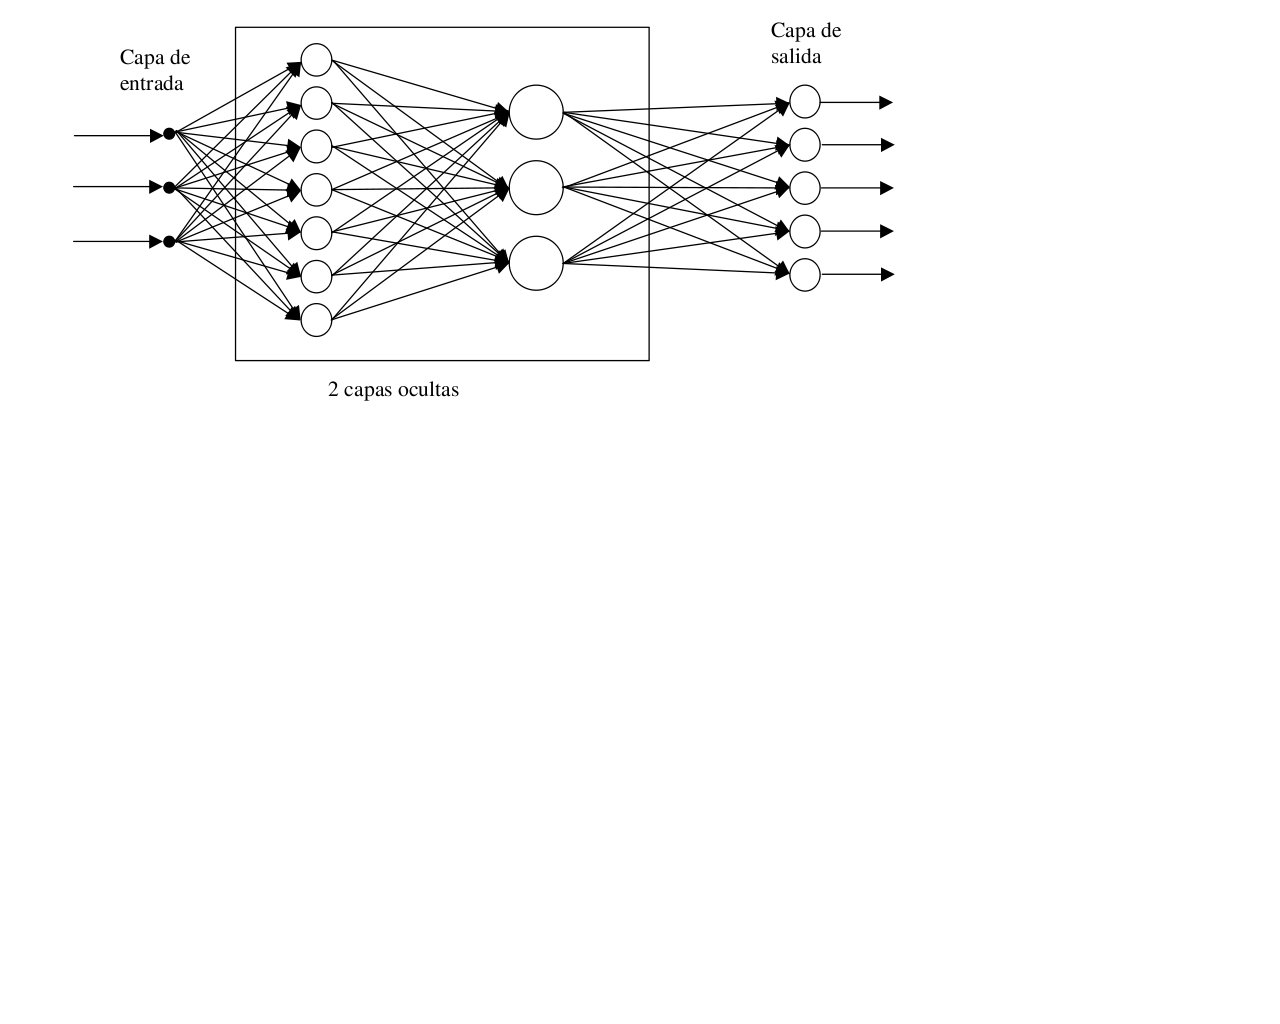
\includegraphics[trim= 0.5cm 22cm 10cm 0cm, clip, width=15cm]{./img/feed-forward.jpg}
\caption{\label{figFeedForward}Red neuronal \emph{feed-forward}.}
\end{figure}

 Las redes neuronales artificiales pueden clasificarse como \emph{feed-forward} (con propagaci\'on hacia delante) o recurrentes dependiendo de su conectividad. Una red es \emph{feed-forward} (figura \ref{figFeedForward}) si existe un m\'etodo de numeraci\'on de las neuronas que cumpla que no existan conexiones desde un nodo hacia otro nodo con un n\'umero m\'as peque\~no que el de nodo de origen. Una red es recurrente (figura \ref{figRecurrente}) si no existe un m\'etodo de numeraci\'on que cumpla tal condici\'on. Para simplificar nuestro trabajo, nos centraremos en las redes \emph{feed-forward}.

\begin{figure}[htb]
\centering
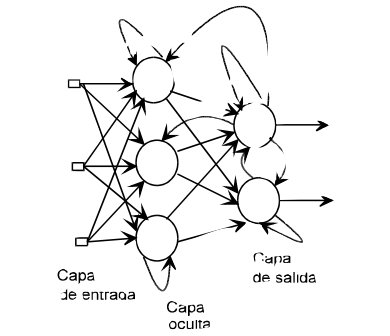
\includegraphics[scale=0.35]{./img/recurrente.jpg}
\caption{\label{figRecurrente}Red neuronal recurrente.}
\end{figure}

 El aprendizaje de las redes neuronales se consigue habitualmente usando ejemplos: suelen tener un entrenamiento supervisado. Se basa en la comparaci\'on directa entre la salida de la red y la salida correcta o deseada. Normalmente se formula el entrenamiento como la minimizaci\'on de una funci\'on de error como el sumatorio del cuadrado del error de la salida respecto de la salida deseada para todos los datos disponibles (que constan de pares de entradas con sus correspondientes salidas deseadas). Un algoritmo de optimizaci\'on basado en el descenso del gradiente como la regla delta generalizada (tambi\'en conocido como algoritmo backpropagation) puede ser usado despu\'es iterativamente para ajustar los pesos y as\'i minimizar el error.

 En nuestro caso, utilizamos aprendizaje por refuerzo y no necesitamos una colecci\'on de ejemplos (aunque se podr\'ia utilizar para calcular el refuerzo). Los pesos los ajustar\'a un algoritmo gen\'etico. La estructura de la red se definir\'a de forma previa para cada problema y s\'olo evolucionar\'an los pesos (y umbrales).
\subsection{Algoritmos gen\'eticos}
\label{sec-2-2}

  \label{basTeoGenet}

Los algoritmos gen\'eticos son m\'etodos sistem\'aticos para la resoluci\'on de problemas de b\'usqueda y optimizaci\'on que aplican a \'estos los principios de la evoluci\'on biol\'ogica: selecci\'on basada en la poblaci\'on, reproducci\'on sexual y mutaci\'on.

 Los algoritmos gen\'eticos son m\'etodos de optimizaci\'on, que tratan de resolver el conjunto de problemas formulados como: hallar (xi,\ldots{},xn) tales que F(xi,\ldots{},xn) sea m\'aximo. En un algoritmo gen\'etico, tras parametrizar el problema en una serie de variables (xi,\ldots{},xn), se codifican en un cromosoma. Todos los operadores utilizados por un algoritmo gen\'etico se aplicar\'an sobre estos cromosomas, o sobre poblaciones de ellos. En el algoritmo gen\'etico va impl\'icito el m\'etodo para resolver el problema; son s\'olo par\'ametros de tal m\'etodo los que est\'an codificados - a diferencia de otros algoritmos evolutivos como la programaci\'on gen\'etica. Hay que tener en cuenta que un algoritmo gen\'etico es independiente del problema, lo cual lo hace un algoritmo robusto, por ser \'util para cualquier problema, pero a la vez d\'ebil, pues no est\'a especializado en ninguno.

 Las soluciones codificadas en un cromosoma compiten para ver cu\'al constituye la mejor soluci\'on (aunque no necesariamente la mejor de todas las soluciones posibles). El ambiente, constituido por las otras camaradas soluciones, ejercer\'a una presi\'on selectiva sobre la poblaci\'on, de forma que s\'olo los mejor adaptados (aquellos que resuelvan mejor el problema) sobrevivan o leguen su material gen\'etico a las siguientes generaciones, igual que en la evoluci\'on de las especies. La diversidad gen\'etica se introduce mediante mutaciones y reproducci\'on sexual. En la Naturaleza lo \'unico que hay que optimizar es la supervivencia, y eso significa a su vez maximizar diversos factores y minimizar otros. Un algoritmo gen\'etico, sin embargo, se usar\'a para optimizar habitualmente para optimizar s\'olo una funci\'on, no diversas funciones relacionadas entre s\'i simult\'aneamente. Este tipo de optimizaci\'on, denominada optimizaci\'on multimodal, tambi\'en se suele abordar con un algoritmo gen\'etico especializado.

 Por lo tanto, un algoritmo gen\'etico consiste en lo siguiente: hallar de qu\'e par\'ametros depende el problema, codificarlos en un cromosoma, y se aplican los m\'etodos de la evoluci\'on: selecci\'on y reproducci\'on sexual con intercambio de informaci\'on y alteraciones que generan diversidad. En las siguientes secciones se ver\'an cada uno de los aspectos de un algoritmo gen\'etico.

 Mediante los operadores de selecci\'on, se eligen los individuos que ser\'an progenitores de la siguiente generaci\'on (o directamente formar\'an parte de ella). Con los operadores de cruza, se generan nuevos individuos mezclando los cromosomas de varios individuos (normalmente, dos). Por \'ultimo, los operadores de mutaci\'on a\~naden cambios aleatorios a los individuos. La funci\'on de fitness nos da una aproximaci\'on de la adaptaci\'on del individuo al medio y \'esta es utilizada por los operadores de selecci\'on.

 En nuestro caso, el cromosoma de cada individuo lo forman los pesos de la red que utiliza ese individuo. Para calcular el fitness del individuo, se construir\'a la red con los pesos del cromosoma y se realizar\'an varias pruebas (para reducir el ruido generado por los posibles factores aleatorios de \'estas) sobre el individuo, sumando las recompensas de todas y obteniendo el citado fitness.
\subsection{Neuro-evoluci\'on}
\label{sec-2-3}

  \label{basTeoNeuro}

 La evoluci\'on se ha aplicado las redes neuronales artificiales en tres niveles muy diferentes: a los pesos de las conexiones, la arquitectura de la red y a las reglas de aprendizaje. La evoluci\'on de los pesos de las conexiones introduce una aproximaci\'on global y adaptable al entrenamiento, especialmente para el aprendizaje por refuerzo o para el entrenamiento de redes recursivas, donde los m\'etodos basados en el gradiente experimentan grandes dificultades. La evoluci\'on de las arquitecturas permite a las redes neuronales adaptar su topolog\'ia a diferentes problemas sin intervenci\'on humana y con esto se consigue un dise\~no autom\'atico de redes neuronales, dado que tanto la arquitectura como los pesos pueden ser evolucionados. La evoluci\'on de las reglas de aprendizaje puede ser considerada como un proceso de \textquotedblleft aprender a aprender\textquotedblright en redes neuronales donde la adaptaci\'on de las reglas de aprendizaje se consigue mediante la evoluci\'on. Tambi\'en puede ser contemplada como un proceso de descubrimiento autom\'atico de nuevas reglas de aprendizaje. Nos centraremos en la evoluci\'on de los pesos de las conexiones, por ser la evoluci\'on que utilizaremos.

 La evoluci\'on de los pesos de las conexiones se puede realizar en el aprendizaje supervisado (con ejemplos) definiendo la funci\'on de fitness como el error global obtenido por la red (invirtiendo el signo), comparando las salidas de la red y la salida deseada para cada ejemplo. Tambi\'en puede utilizar para el aprendizaje por refuerzo definiendo una funci\'on de fitness distinta.

 En general, los pasos a seguir son dos: decidir la codificaci\'on de los pesos de las conexiones (si se har\'a mediante cadenas binarias o no) y la ejecuci\'on del algoritmo gen\'etico propiamente dicho. Para el primer paso, las opciones m\'as extendidas son la representaci\'on binaria y la representaci\'on con n\'umeros reales.

   El algoritmo gen\'etico can\'onico siempre usa cadenas de bits para codificar las diferentes soluciones. Por ello, algunos trabajos tempranos de evoluci\'on de los pesos de las conexiones siguen esta aproximaci\'on \cite[Yao99]{Yao99}. Las ventajas son la f\'acil aplicaci\'on de los operadores gen\'eticos y su posible implementaci\'on digital. Habr\'ia que elegir la representaci\'on de los n\'umeros reales. Aqu\'i hay un compromiso para la precisi\'on con que se quieran representar los n\'umeros reales. Si se usan muy pocos bits para representar cada conexi\'on, el entrenamiento puede fallar porque algunas combinaciones de pesos no se pueden aproximar con suficiente precisi\'on por valores discretos. Por otra parte, si se usan demasiados bits, los cromosomas que representen a redes neuronales grandes se volver\'an demasiado largos y la evoluci\'on en proceso resultar\'a muy ineficiente.

 Por su parte, en la representaci\'on con n\'umeros reales, los cromosomas se codifican como vectores de n\'umeros reales con tantos elementos como conexiones. Los operadores gen\'eticos no se pueden aplicar directamente sobre los bits y han de ser dise\~nados de nuevo. Esto puede ser una ventaja, pues, por ejemplo, el operador de mutaci\'on podr\'ia tener una distribuci\'on gaussiana (u otra funci\'on) en lugar de mutar un bit cualquiera sin tener en cuenta su peso en la construcci\'on del n\'umero.

\begin{figure}[t]
\begin{minipage}{0.45\textwidth}
    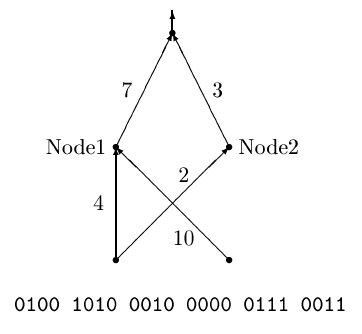
\includegraphics [width=7.20cm]{./img/grafo1.jpg}
  \caption {Red neuronal y su codificaci\'on binaria (asumiendo que se usan 4 bits para representar cada n\'umero real).}\label{figGrafo1}
\end{minipage}
\begin{minipage}{0.10\textwidth}
\hfill
\end{minipage}
\begin{minipage}{0.45\textwidth}
    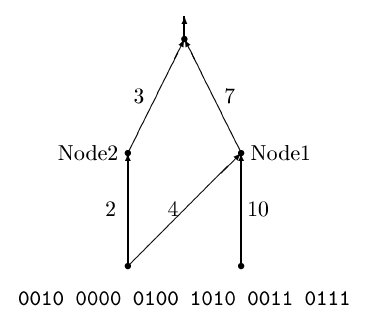
\includegraphics [width=7.20cm]{./img/grafo2.jpg}
  \caption{Red equivalente con codificaci\'on alternativa.}\label{figGrafo2}
\end{minipage}
\end{figure}

 Uno de los problemas a los que se enfrenta la evoluci\'on de redes neuronales es el problema de la permutaci\'on. Es causado por el mapeado ``muchos-a-uno'' desde la representaci\'on en el cromosoma a la red que es construida. Con dos cromosomas distintos se pueden generar redes equivalentes como se muestra en las figuras \ref{figGrafo1} y \ref{figGrafo2}. Se puede solucionar dando m\'as importancia al operador de mutaci\'on que al de cruza (que es el que sufre con este problema) o con otros m\'etodos matem\'aticos \cite[Gomez, Miikkulainen 2003]{GomezMiikkulainen2003}. 

\newpage
\section{An\'alisis del problema}
\label{sec-3}

  \label{analisis}
\subsection{Fortalezas y deficiencias}
\label{sec-3-1}

  \label{anaFortYDeb}

 Tanto las redes neuronales como los algoritmos gen\'eticos tienen fortalezas que nuestro m\'etodo aprovecha y debilidades que se pueden, en parte, minimizar por la combinaci\'on de ambos m\'etodos.
\subsubsection{Redes neuronales}
\label{sec-3-1-1}

  \label{anaFortYDebRedes}

 Las redes neuronales con conexi\'on hacia delante en general son un importante m\'etodo de aproximaci\'on de funciones [Kim, 1992]. El perceptr\'on multicapa es un tipo de red neuronal con conexiones hacia delante. La topolog\'ia de un perceptr\'on multicapa esta definida por un conjunto de capas ocultas, una capa de entrada y una de salida. No existen restricciones sobre la funci\'on de activaci\'on aunque en general se suelen utilizar funciones sigmoideas. Existen demostraciones te\'oricas [Funahashi, 1989] de que un perceptr\'on multicapa cuya funci\'on de activaci\'on sea no constante, acotada y mon\'otona creciente es un aproximador universal de funciones. En [Hornik et alt, 1989] se llega a un resultado similar utilizando funciones de activaci\'on sigmoideas, no necesariamente continuas. Esto es un punto muy fuerte de las redes neuronales. 

 Adem\'as, constituyen buena una herramienta para la construcci\'on de agentes pues s\'olo hay que codificar las entradas y las salidas de la red como las del agente y el tiempo de ejecuci\'on de la red s\'olo depende de la topolog\'ia de \'esta (para una topolog\'ia dada, es constante).

 Algunas deficiencias del algoritmo back-propagation son su baja adaptabilidad, la alta dependencia de los par\'ametros del algoritmo, el estancamiento en m\'inimos locales, la posibilidad de par\'alisis y la alta dependencia de las condiciones iniciales.
\begin{listaDefiniciones}

 \item[Adaptabilidad] El algoritmo tiene como premisa la utilizaci\'on de una funci\'on de activaci\'on derivable [Walker, 1995]. Al hacer uso de la derivada de la funci\'on de activaci\'on, es condici\'on necesaria para la aplicaci\'on del algoritmo que la misma sea continua y derivable en todo el dominio de aplicaci\'on [Wilson, 1994]. Esto impide la utilizaci\'on del m\'etodo en otras topolog\'ias donde la funci\'on de activaci\'on presenta discontinuidades.

 Este problema suele encontrarse en varios m\'etodos de entrenamiento, los cuales son desarrollados para una determinada topolog\'ia y sus resultados, en general, no son extensibles directamente a otras topolog\'ias. Es necesario adaptar los m\'etodos para aplicarlos a otras topolog\'ias.

\item[Dependencia de par\'ametros del algoritmo] Los algoritmos de gradiente descendente hacen uso de una tasa de aprendizaje que idealmente deber\'ia ser infinitesimal. De esta manera, mediante peque\~nos ajustes de los pesos sin\'apticos el algoritmo converge hacia un m\'inimo. El uso de tasas de aprendizaje muy peque\~nas hace que el algoritmo tenga una convergencia estable hacia un m\'inimo, aunque el tiempo necesario para alcanzarlo puede llegar a ser muy alto. Como consecuencia de lo dicho anteriormente, y con el objetivo de disminuir el tiempo de convergencia del algoritmo, en la pr\'actica se suelen utilizar tasas de aprendizajes mayores a las te\'oricas. El aumento de la tasa de aprendizaje disminuye el tiempo de convergencia, pero tiene un efecto contraproducente: el algoritmo comienza a oscilar en torno a un m\'inimo, disminuyendo la probabilidad de alcanzarlo. El efecto de oscilaci\'on puede reducirse mediante la adici\'on de una tasa de momento, como se describi\'o en el cap\'itulo 3, pero no puede eliminarse.

 El algoritmo backpropagation es muy dependiente de los par\'ametros mencionados previamente. Dependiendo de la selecci\'on de par\'ametros realizadas el resultado de la aplicaci\'on del algoritmo ser\'a exitosa o no [Liu et alt, 2004]. Peque\~nas variaciones sobre los par\'ametros del algoritmo pueden conducir a resultados diferentes. El principal problema es que no existe un m\'etodo general que permita establecer el valor de estos par\'ametros [Branke, 1995]. Los par\'ametros que aseguran la convergencia para un determinado problema pueden no ser aplicables a otro problema. De esta manera, la selecci\'on de los par\'ametros del algoritmo se realiza en base a la experiencia del dise\~nador, y se realiza un refinamiento de los mismos mediante mecanismos de prueba y error. Esto produce un aumento en el tiempo total de dise\~no y entrenamiento de la red.

\item[M\'inimos locales] La superficie que define la funci\'on de error E (ecuaci\'on 8) en base a los par\'ametros de la red neuronal es compleja y esta llena de valles y colinas. Debido a la utilizaci\'on del gradiente para encontrar el m\'inimo de dicha funci\'on de error se corre el riesgo de que el proceso de entrenamiento quede atrapado en un m\'inimo local [Sutton, 1986]. Esta situaci\'on no es deseable, fundamentalmente si dicho m\'inimo esta localizado lejos del m\'inimo global.

 Existen algunos mecanismos para evitar que esto suceda. Una posible soluci\'on para evitar que el entrenamiento quede atrapado en un m\'inimo local es aumentar el n\'umero de neuronas ocultas de la red. Este mecanismo puede ayudar en aquellos casos en los que la red tiene escaso poder de representaci\'on interna, y no es capaz de distinguir entre dos patrones diferentes, proporcionando una misma salida para ambos patrones. Al aumentar el n\'umero de neuronas ocultas la red posee mayor cantidad de par\'ametros libres y puede conseguir una mejor representaci\'on interna.

 Otros mecanismos que ayudan a disminuir los efectos de este problema son la adici\'on de una tasa de momento al proceso de entrenamiento, utilizar una tasa de aprendizaje decreciente a lo largo del proceso, partir de otras configuraciones iniciales de la red, a\~nadir ruido al m\'etodo de gradiente, etc.

\item[Par\'alisis] El fen\'omeno de par\'alisis, tambi\'en conocido como saturaci\'on, se produce cuando la entrada total a una neurona de la red toma valores muy altos, ya sean positivos o negativos. Al utilizar funciones de activaci\'on sigmoidales, la funci\'on de activaci\'on posee dos as\'intotas horizontales. Si la entrada de la neurona alcanza un valor alto, la funci\'on de activaci\'on se satura y alcanza un valor de activaci\'on m\'aximo o m\'inimo.

 Cuando la funci\'on de activaci\'on se satura su derivada tiende a hacerse nula, haciendo que los par\'ametros de la red permanezcan invariables y, como consecuencia, la suma de los errores locales permanece constante por un largo periodo de tiempo [Kr\"ose y van der Smagt, 1993]. Aunque esta situaci\'on se suele confundir con un m\'inimo local, pues el error permanece invariable, en este caso es posible que despu\'es de un cierto tiempo el error comience nuevamente a decrecer.

 El fen\'omeno de par\'alisis del perceptr\'on multicapa ocurre fundamentalmente cuando los par\'ametros de la red toman valores muy altos. Un mecanismo para evitar esto consiste en partir de valores iniciales bajos.

\item[Condiciones iniciales] El conjunto de pesos iniciales de la red neuronal generalmente se selecciona de manera aleatoria. Sin embargo, el algoritmo backpropagation es muy dependiente de las condiciones iniciales seleccionadas [Kolen, 1991]. Peque\~nas variaciones realizadas sobre las condiciones iniciales pueden llevar a grandes diferencias en el tiempo de convergencia del algoritmo.
\end{listaDefiniciones}

 A esto hay que a\~nadir que los algoritmos de gradiente requieren entrenamiento supervisado (normalmente, no funcionan para el aprendizaje por refuerzo) y que las conexiones sean hacia delante (la retro-propagaci\'on del error no se puede aplicar en redes recurrentes). 

 Usando un algoritmo gen\'etico como m\'etodo de entrenamiento de la red, se solucionan algunos de estos problemas y otros se mitigan en cierto grado. Con el algoritmo gen\'etico, se puede usar el aprendizaje por refuerzo y se pueden entrenar redes recurrentes sin problema. No se tienen requerimientos para la funci\'on de activaci\'on, por lo que aumenta su adaptabilidad. Se cambia la dependencia de los par\'ametros de ese algoritmo y ahora depende de los par\'ametros del algoritmo gen\'etico, estos par\'ametros son m\'as flexibles y se pueden alterar en medio del entrenamiento. El algoritmo gen\'etico es mucho menos tendente a estancarse en m\'inimos locales porque no utiliza la informaci\'on del gradiente y porque explora varios puntos (tantos como individuos tenga la poblaci\'on) del espacio de b\'usqueda simult\'aneamente. El fen\'omeno de saturaci\'on se produce cuando una neurona alcanza un m\'aximo o un m\'inimo. En este caso, la derivada de la funci\'on de activaci\'on se hace nula, y los pesos de la red permanecen invariables. Como el m\'etodo propuesto no hace uso de la derivada de la funci\'on de activaci\'on, el efecto de este fen\'omeno es completamente eliminado. Los valores iniciales de los pesos tambi\'en pueden afectar al algoritmo gen\'etico, en especial si son muy altos (ya sean positivos o negativos), pero existen experimentos que permiten afirmar que el m\'etodo propuesto es menos dependiente de los valores iniciales que el algoritmo backpropagation \cite[Bertona2005]{Bertona2005}.
\subsubsection{Algoritmos gen\'eticos}
\label{sec-3-1-2}

  \label{anaFortYGene}

Un algoritmo gen\'etico es independiente del problema, lo cual lo hace un algoritmo robusto, por ser \'util para cualquier problema, pero a la vez d\'ebil, pues no est\'a especializado en ninguno. Hay que elegir la codificaci\'on de los cromosomas para cada caso concreto. Sin embargo, con nuestro m\'etodo siempre c\'odificaremos los cromosomas de manera similar (con una red neuronal) y s\'olo ser\'a necesario definir la funci\'on de fitness, elegir la topolog\'ia de la red, codificar las entradas y las salidas. Aunque la codificaci\'on de \'estas pueda admitir varias posibilidades (y algunas puedan ser m\'as ventajosas que otras) la red debe aprender a interpretar las correctas relaciones entre entradas y salidas por s\'i misma.
\subsection{Objetivos}
\label{sec-3-2}

  \label{anaObjetivos}

En el presente proyecto se pretende construir una librer\'ia de programaci\'on en C++ para la utilizaci\'on de redes neuronales con entrenamiento mediante algoritmos gen\'eticos. Se quiere que sea lo m\'as flexible posible en cuanto a la estructura de la red, para poder, en un futuro, determinar la topolog\'ia tambi\'en de forma gen\'etica. Por tanto, con la librer\'ia implementada debe ser posible crear una cualquier red con una arquitectura arbitraria. Deben ser posibles conexiones recurrentes y conectar capas con tipos de datos diferentes (por ejemplo, que una capa cuya salida son n\'umeros en coma flotante debe poder usar como entrada una capa que tiene bits como salida).

 Como los entrenamientos pueden ser costosos en tiempo de ejecuci\'on, la librer\'ia debe estar paralelizada internamente al menos para la ejecuci\'on de redes neuronales. Esta paralelizaci\'on debe poder aprovecharse por los sistemas m\'as extendidos para que pueda ser utilizada en proyectos que aprovechen la computaci\'on voluntaria.

 Adem\'as, se probar\'a la librer\'ia en casos concretos con el fin de contestar a las siguientes cuestiones:

\begin{enumerate}
 
 \item  ?`Qu\'e ventajas en el rendimiento se pueden obtener gracias a la paralelizaci\'on?

 \item  ?`Se puede simplificar la estructura de las redes neuronales para mejorar la paralelizaci\'on? ?`Qu\'e efecto tienen las funciones de tipo escal\'on (que permiten codificar la salida de cada neurona como un bit en vez de como un n\'umero real) tanto en el rendimiento como en el aprendizaje? ?`Qu\'e efecto tiene la codificaci\'on de los pesos en estructuras discretas (en lugar de n\'umeros reales) tanto en el rendimiento como en el aprendizaje?

 \item  ?`Qu\'e operadores gen\'eticos resultan m\'as adecuados para el entrenamiento en diferentes problemas? ?`Qu\'e valores de los par\'ametros del algoritmo gen\'etico resultan m\'as adecuados para el entrenamiento en diferentes problemas?

 \item  ?`Para qu\'e tipo de problemas resulta m\'as adecuado el m\'etodo propuesto? 

\end{enumerate}

\newpage
\section{Dise\~no e implementaci\'on}
\label{sec-4}

  \label{diseno}
\subsection{Implementaciones paralelas de las redes neuronales}
\label{sec-4-1}

  \label{disenoParal}
\subsubsection{Utilizaci\'on del coprocesador XMM}
\label{sec-4-1-1}

  \label{disenoParalXMM}
\subsubsection{Utilizaci\'on de la arquitectura CUDA}
\label{sec-4-1-2}

  \label{disenoParalCUDA}
\subsection{Dise\~no del algoritmo gen\'etico}
\label{sec-4-2}

  \label{disenoGene}
\subsection{Interfaz del programador}
\label{sec-4-3}

  \label{disenoInterfProgr}
\newpage
\section{Experimentaci\'on}
\label{sec-5}

  \label{experimentacion}
\subsection{Tareas de clasificaci\'on}
\label{sec-5-1}

  \label{}
\subsection{Juegos de estrategia abstractos}
\label{sec-5-2}

  \label{}
\newpage
\section{Resultados}
\label{sec-6}

  \label{resultados}
\subsection{Rendimiento}
\label{sec-6-1}

  \label{rendimiento}

En esta sección se analizan resultados de rendimiento en tiempo de ejecución.
\subsubsection{Rendimiento de las implementaciones paralelas de red neuronal}
\label{sec-6-1-1}

  \label{rendImpl}

En esta sección se presentan los resultados en tiempo de ejecución de los métodos que se ejecutan de forma diferente con cada implementación.
\paragraph{Acumulación de resultados}
\label{sec-6-1-1-1}


En la figura \ref{grafImplCalculate}, puede apreciarse que la implementación con instrucciones SSE2 de ensamblador para utilizar el coprocesador XMM es muy superior a la implementación de referencia en lenguaje C, especialmente para los tipos de Buffer BIT y SIGN.

\begin{figure}[htb]
\centering
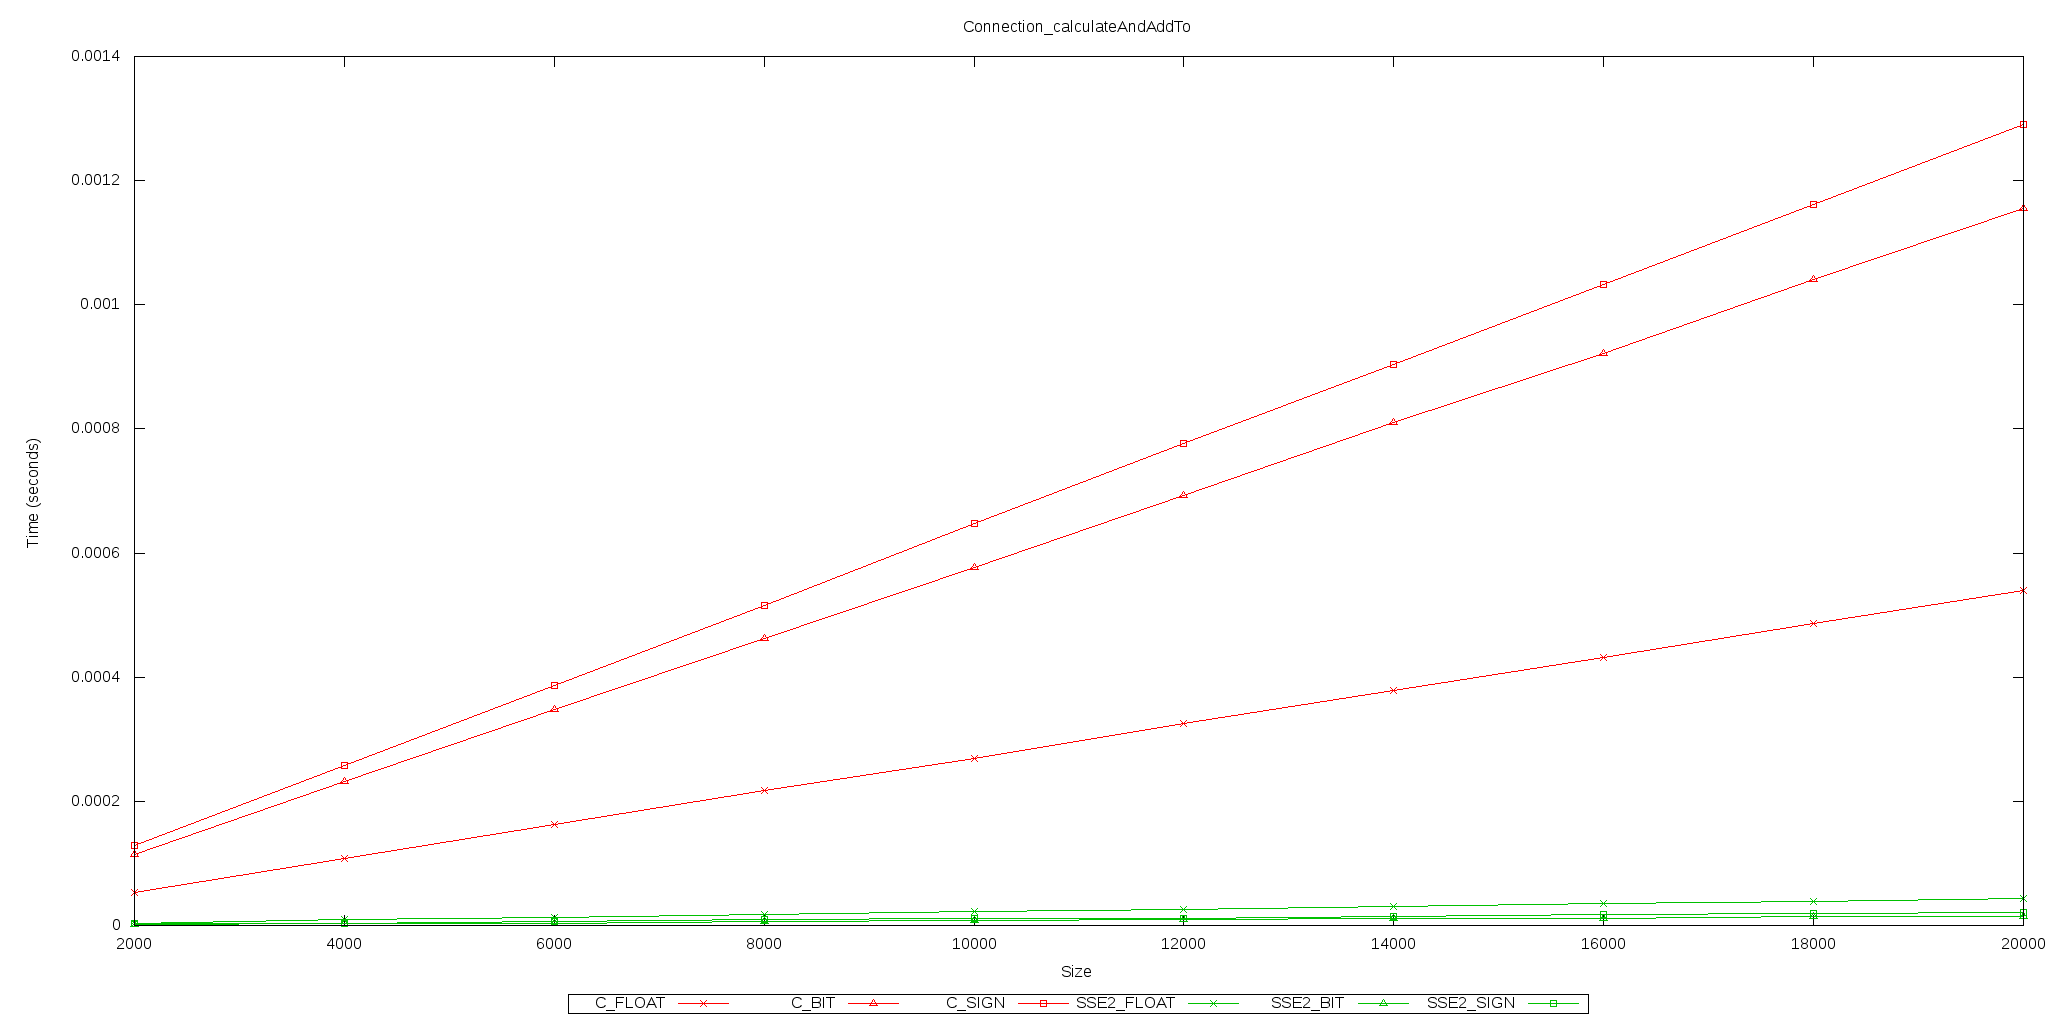
\includegraphics[width=\textwidth]{./img/Connection_calculateAndAddTo.png}
\caption{\label{grafImplCalculate}Método de acumulación de resultados (Connection::calculateAndAdd).}
\end{figure}
\newpage
\paragraph{Activación}
\label{sec-6-1-1-2}


De la figura \ref{grafImplActivation} se extraen varias conclusiones. No mucha diferencia de rendimiento entre las implementaciones y prácticamente ninguna cuando las neuronas son de tipo FLOAT. Esto era de esperar porque ambas implementaciones son idénticas: no se han hecho optimizaciones SSE2 para la función de activación para el tipo FLOAT.

Para los tipos BIT y SIGN, la implementación en C es ligeramente más rápida que para el tipo FLOAT y la  escrita en SSE2 es ligeremante más lenta que la FLOAT. En la implementación SSE2 de BIT y SIGN no se ponen los bits en el orden normal, si no en la representación especial de SSE2, para que el método de acumulación de resultados pueda ser óptimo.

\begin{figure}[htb]
\centering
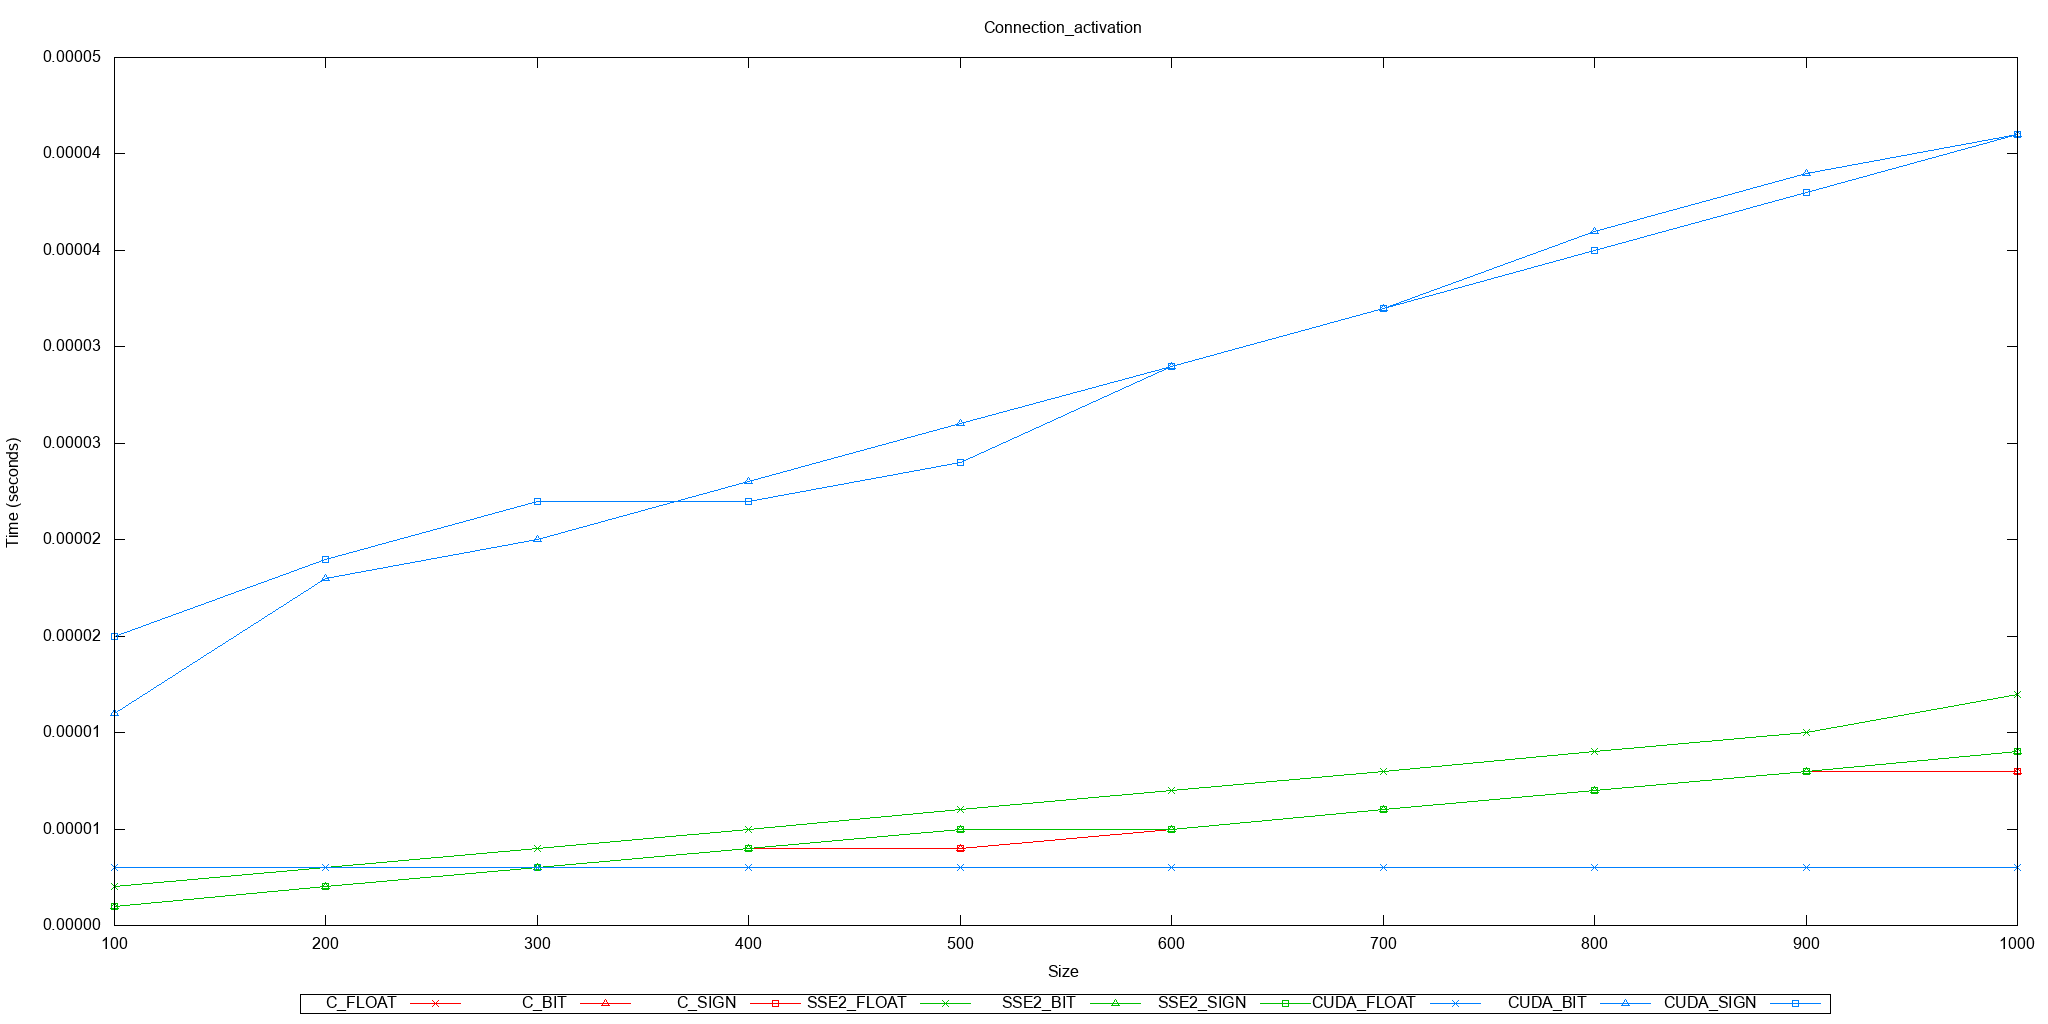
\includegraphics[width=\textwidth]{./img/Connection_activation.png}
\caption{\label{grafImplActivation}Método que ejecuta la función de activación para las salidas de una capa (Connection::activation).}
\end{figure}
\newpage
\paragraph{Funciones de activación}
\label{sec-6-1-1-3}


Si en la figura \ref{grafImplActivation} se comparaba el rendimiento de los distintos tipos de neurona (BIT, SIGN y FLOAT con la función de activación IDENTITY), en la figura \ref{grafImplActivationFunc} se comparan los rendimientos de los distintos tipos de funciones para el tipo de neurona FLOAT. Con el tipo de neurona BIT, la función de activación siempre es BINARY$_{\mathrm{STEP}}$ y con el tipo SIGN la activación siempre es BIPOLAR$_{\mathrm{STEP}}$, por ello podemos excluir estos tipos de esta gráfica. Además, la implementación SSE2 de la activación para FLOAT es idéntica a la de C, por lo que tampoco se muestran los resultados de la activación SSE2 en este caso.

Se puede ver como, en general, la función más lenta es la sigmoide, seguida de la sigmoide bipolar. La tangente hiperbólica sólo es ligeramente más lenta que el resto, cuyo rendimiento es similar al de la función identidad (que no hace nada).

\begin{figure}[htb]
\centering
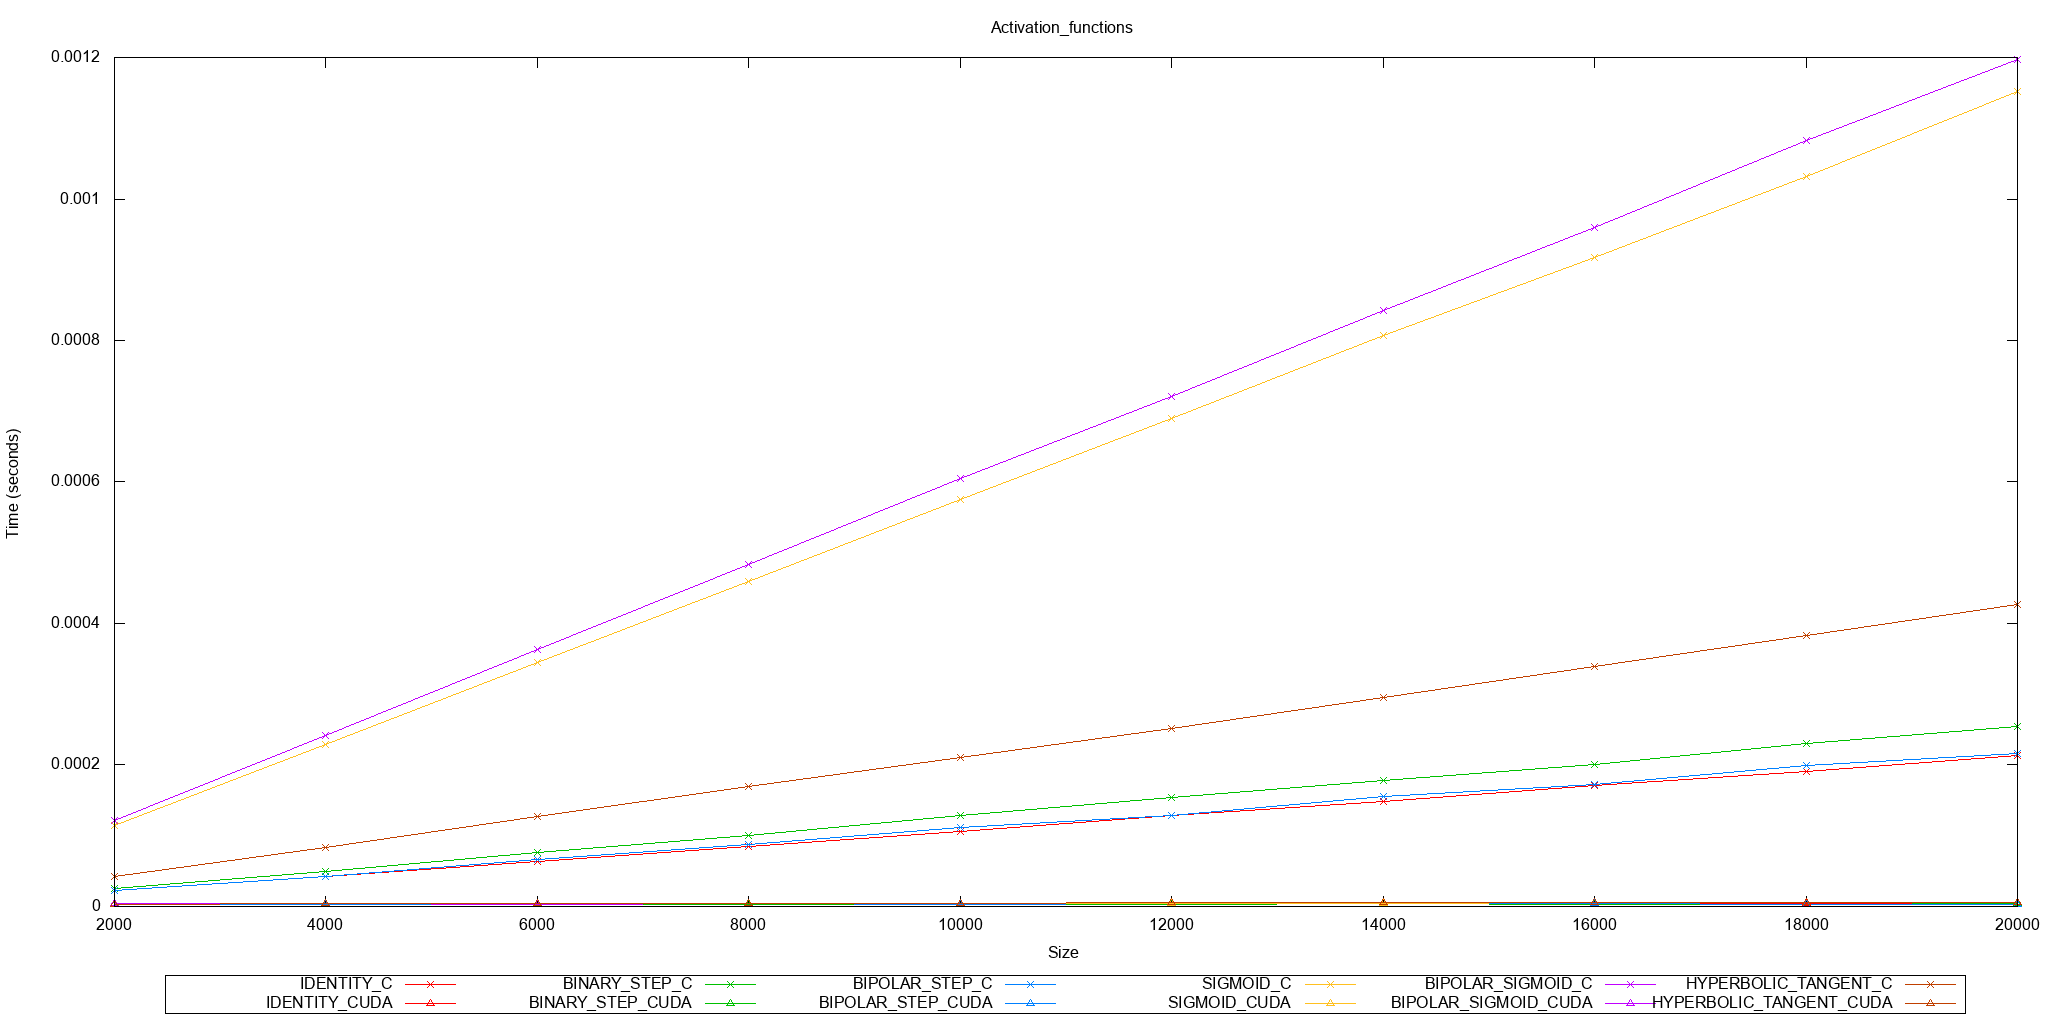
\includegraphics[width=\textwidth]{./img/Activation_functions.png}
\caption{\label{grafImplActivationFunc}Método que ejecuta la función de activación para las salidas de una capa (Connection::activation) con tipo de Buffer FLOAT y las diferentes funciones de activación implementadas.}
\end{figure}
\newpage
\paragraph{Cruza}
\label{sec-6-1-1-4}


No hay una diferencia sustancial de rendimiento entre las diferentes implementaciones y tipos de neuronas para el operador genético de crossover, como se muestra en la figura \ref{grafImplCrossover}. Como el método de activación, la cruza de SSE2 se ve ligeramente penalizada al traducir el vector de bits con los pesos a cruzar para que tenga se adapte a la posición especial de los pesos en SSE2.

\begin{figure}[htb]
\centering
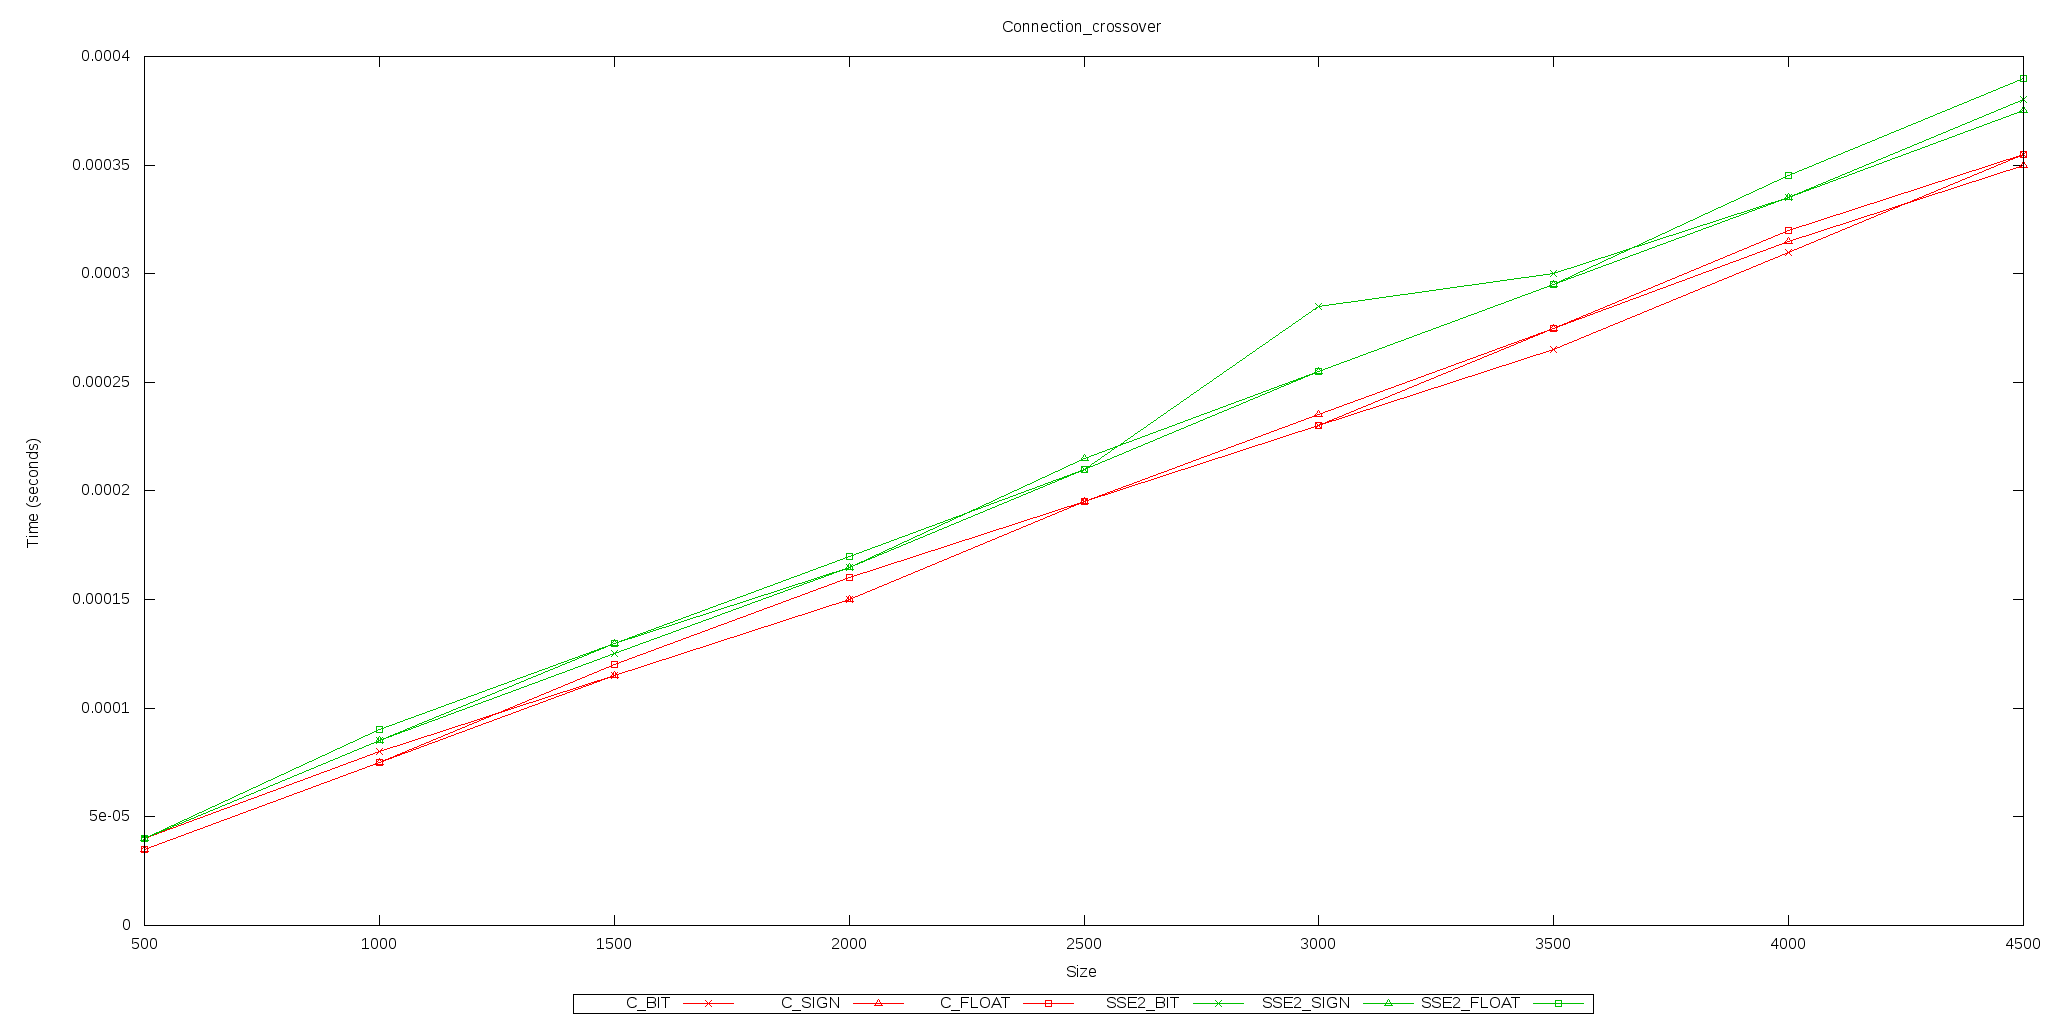
\includegraphics[width=\textwidth]{./img/Connection_crossover.png}
\caption{\label{grafImplCrossover}Método que implementa el operador de crossover para dos conexiones dadas (Connection::crossover).}
\end{figure}
\newpage
\paragraph{Mutación}
\label{sec-6-1-1-5}


De la figura \ref{grafImplMutation} se puede deducir que el operador de mutación tiene un coste mínimo y constante respecto al tamaño de la conexión para todas las implementaciones.

\begin{figure}[htb]
\centering
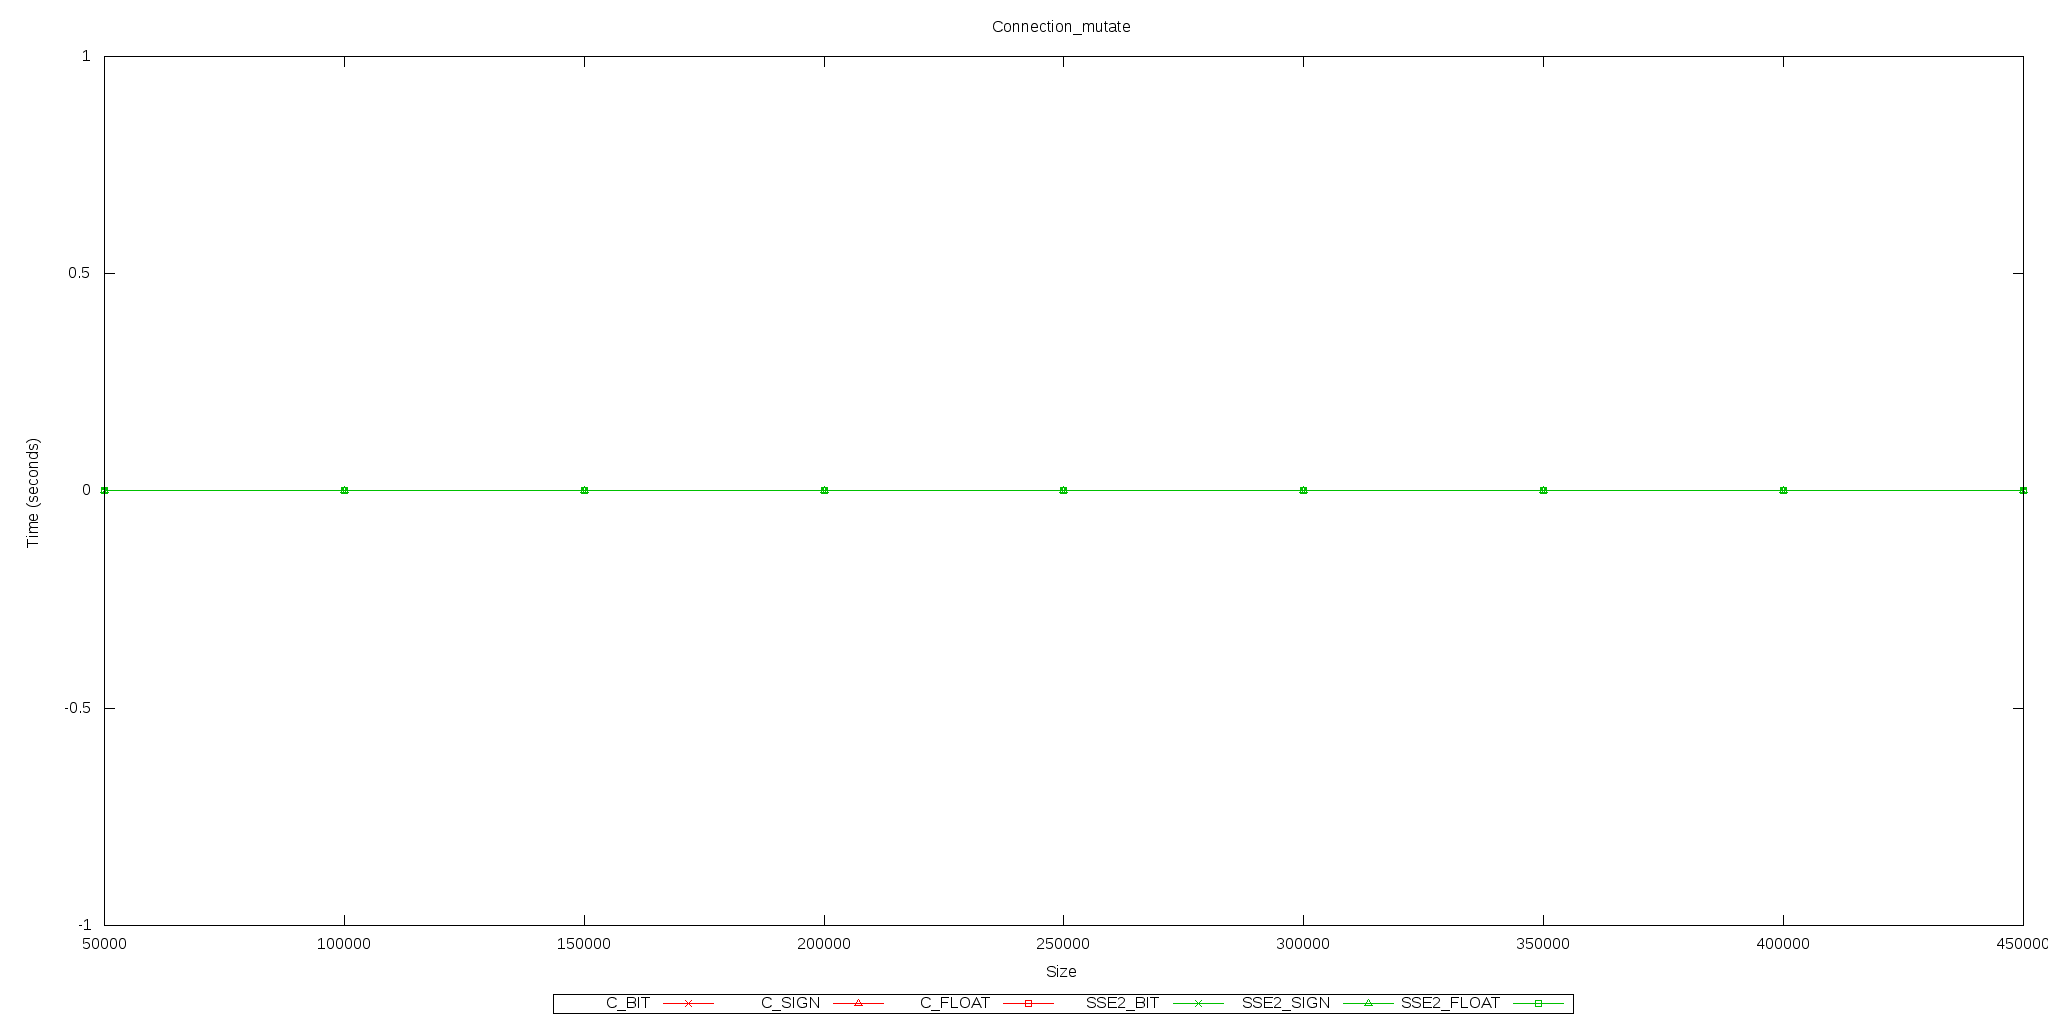
\includegraphics[width=\textwidth]{./img/Connection_mutate.png}
\caption{\label{grafImplMutation}Método que implementa el operador genético de mutación (Connection::mutate).}
\end{figure}
\newpage
\paragraph{Olvido}
\label{sec-6-1-1-6}


De manera similar a la operación de mutación, el olvido (figura \ref{grafImplReset}) tiene un coste constante y mínimo.

\begin{figure}[htb]
\centering
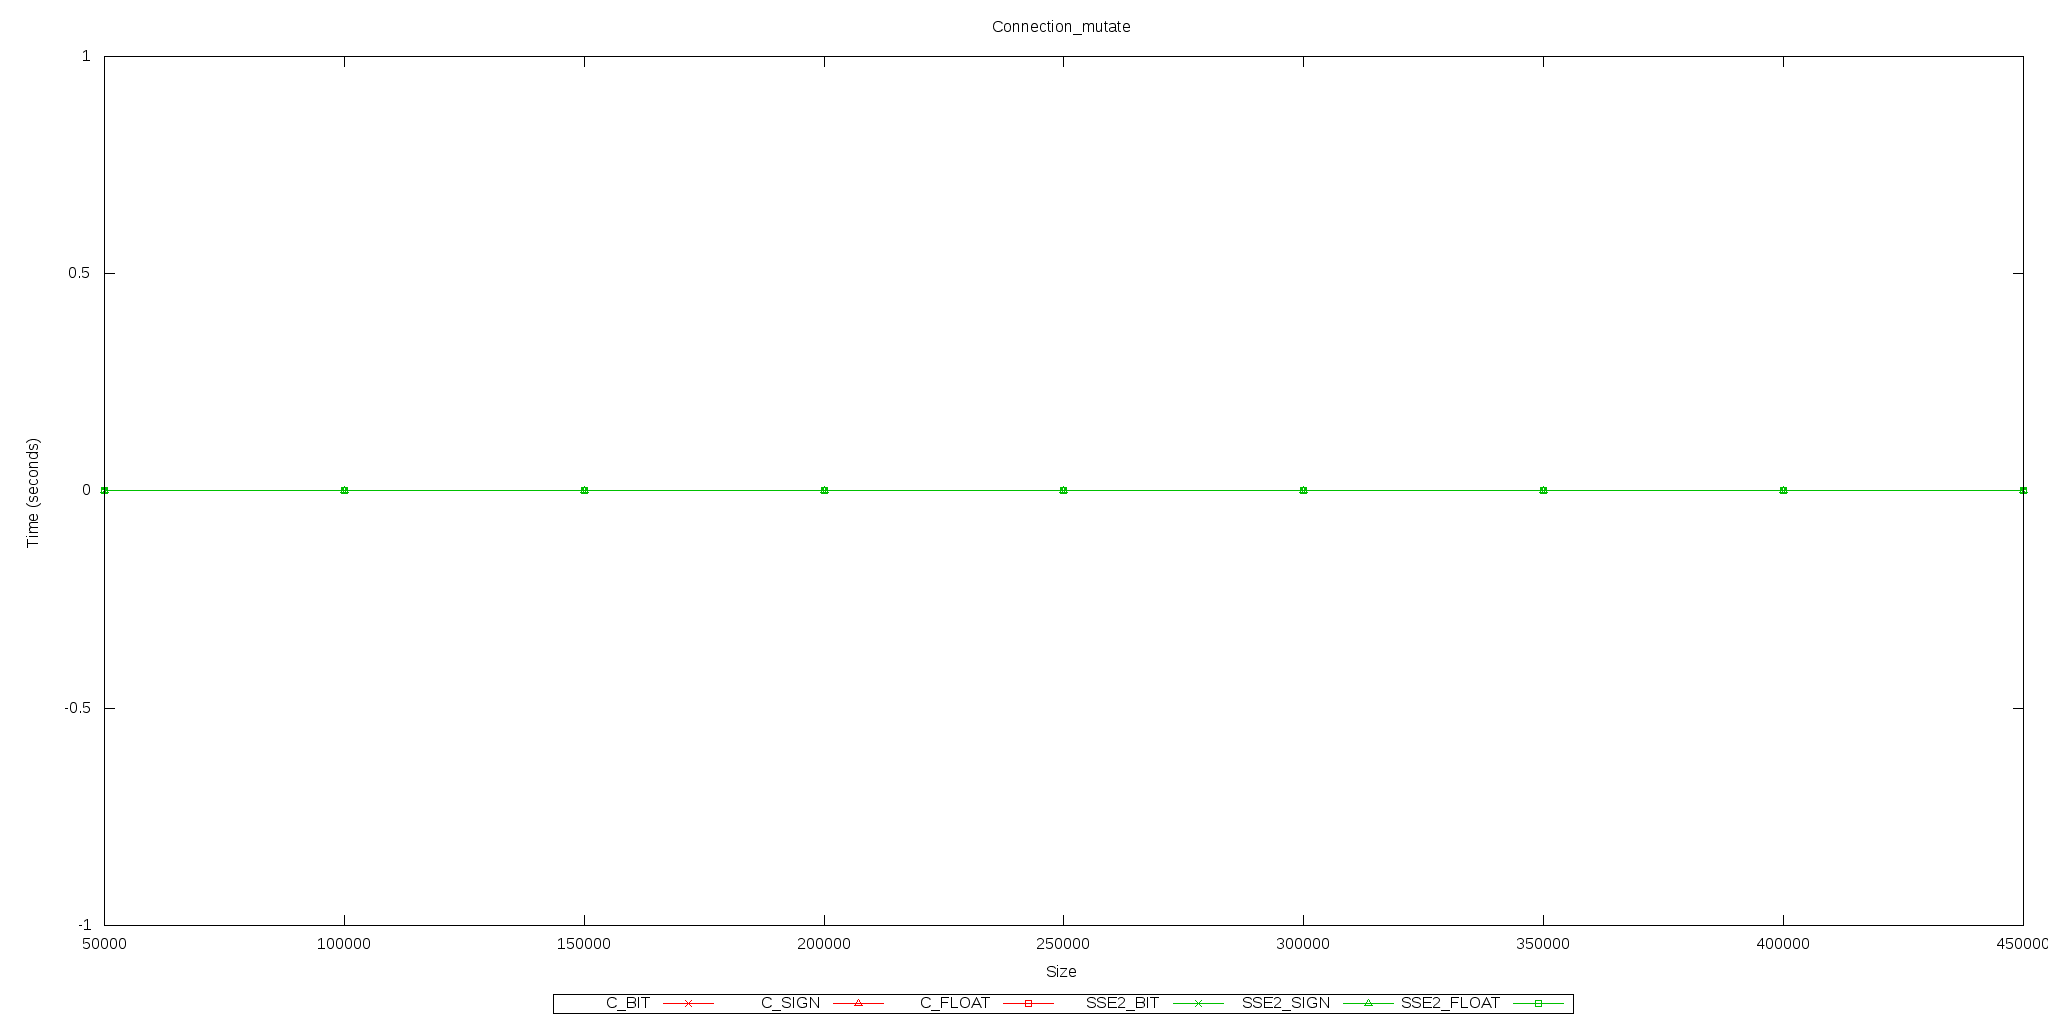
\includegraphics[width=\textwidth]{./img/Connection_reset.png}
\caption{\label{grafImplReset}Método que implementa el operador genético de olvido (Connection::reset).}
\end{figure}
\newpage
\paragraph{Copiar desde y hacia Interfaz}
\label{sec-6-1-1-7}


Estos métodos se usan para recibir entradas y sacar salidas al exterior de la red. Las interfaces sirven para independizar la red de la implementación concreta escogida. Cada implementación debe mapear correctamente desde la representación genérica (Interfaz) hacia su propia representación interna (figura \ref{grafImplCopyFrom}) de los datos y viversa (figura \ref{grafImplCopyTo}).

\begin{figure}[htb]
\centering
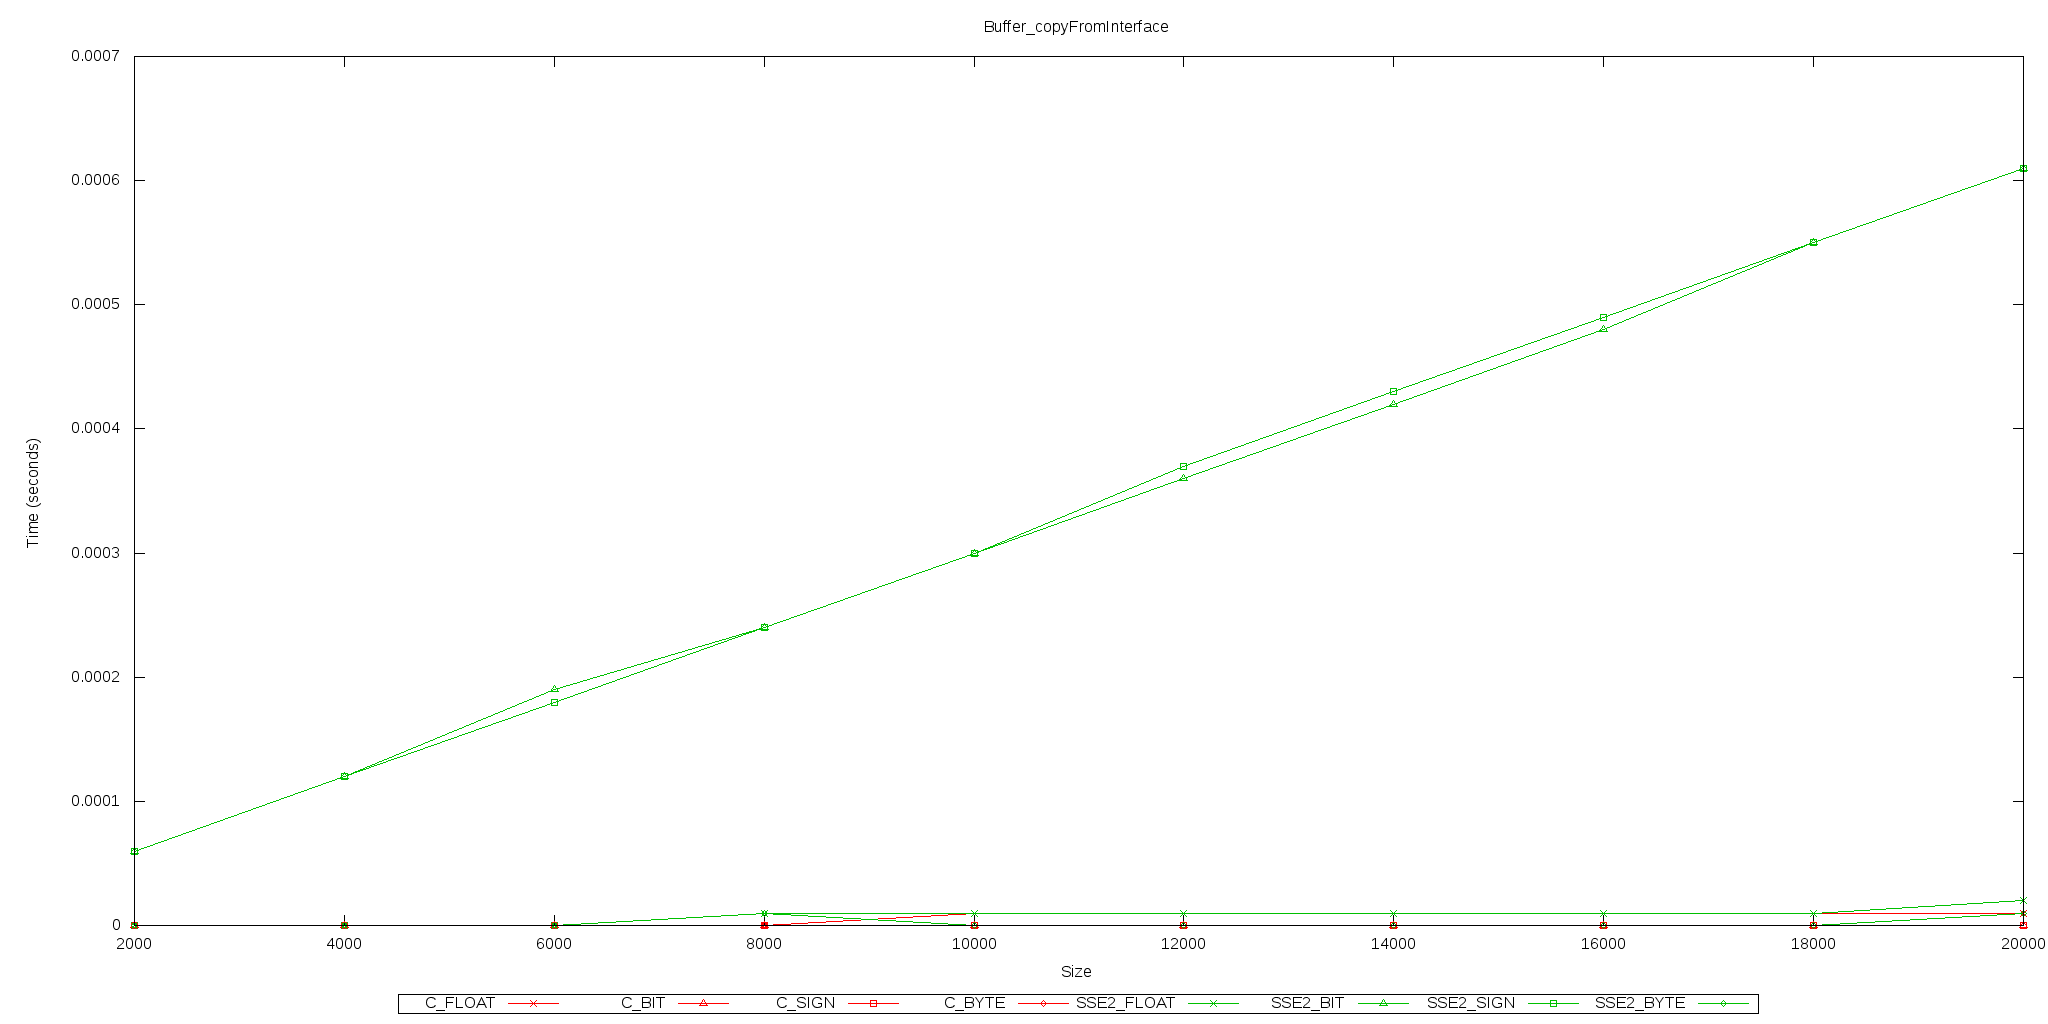
\includegraphics[width=\textwidth]{./img/Buffer_copyFromInterface.png}
\caption{\label{grafImplCopyFrom}Método que implementa la copia a un Buffer con una implementación determinada desde un Buffer genérico de la clase Interfaz (Buffer::copyFromInterface).}
\end{figure}

En ambos casos se observa que el coste es muy pequeño excepto para la implementación SSE2 de los tipos BIT y SIGN, por razones similares a las de Activación.

\begin{figure}[htb]
\centering
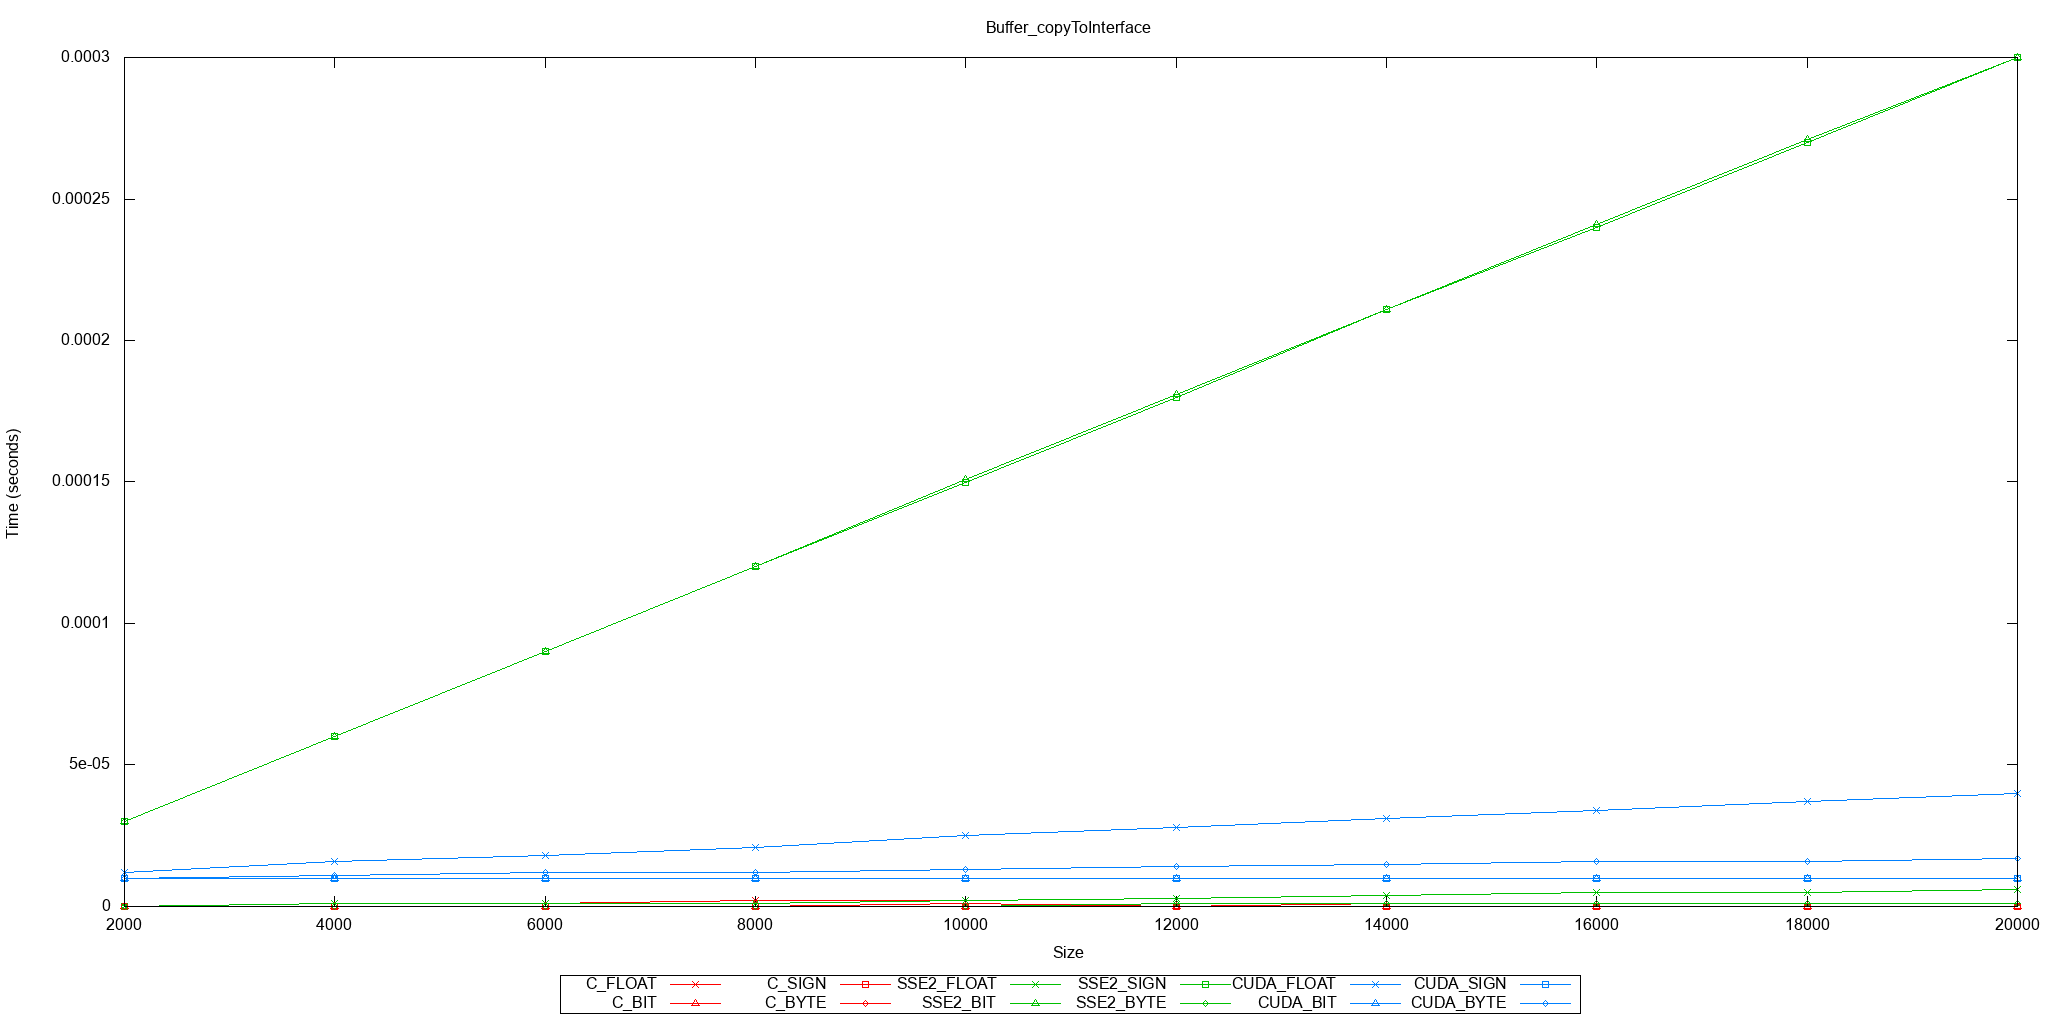
\includegraphics[width=\textwidth]{./img/Buffer_copyToInterface.png}
\caption{\label{grafImplCopyTo}Método que implementa la copia de un Buffer con una implementación determinada a un Buffer genérico de la clase Interfaz (Buffer::copyToInterface).}
\end{figure}
\newpage
\subsubsection{Rendimiento de los diferentes operadores genéticos}
\label{sec-6-1-2}

   \label{rendOperadores}

En esta sección se cronometran los operadores genéticos. Algunos ya se habían analizado en la sección \ref{rendImpl}, pero a un nivel más bajo, del que dependen las implementaciones. Ahora lo que nos interesa es principalmente el coste de los operadores dependiendo de las diferentes formas de usarlo a más alto nivel. Nos abstraemos por ello de la implementación concreta y usamos la implementación SSE2 para todas estas pruebas.
\paragraph{Selección}
\label{sec-6-1-2-1}


figura \ref{rendGenSelect}

Aunque no se aprecia bien en la figura \ref{rendGenSelect}, las selecciones de ruleta y truncado tienen un coste mínimo y bastante independiente tanto del tamaño total de la población como del número de individuos a seleccionar en comparación con los otros dos esquemas de selección. La selección por ranking es la más costosa y además la que más depende del tamaño total de la población. La selección por torneo es algo menos costosa y depende más del tamaño del torneo que del tamaño total de la población.

\begin{figure}[htb]
\centering
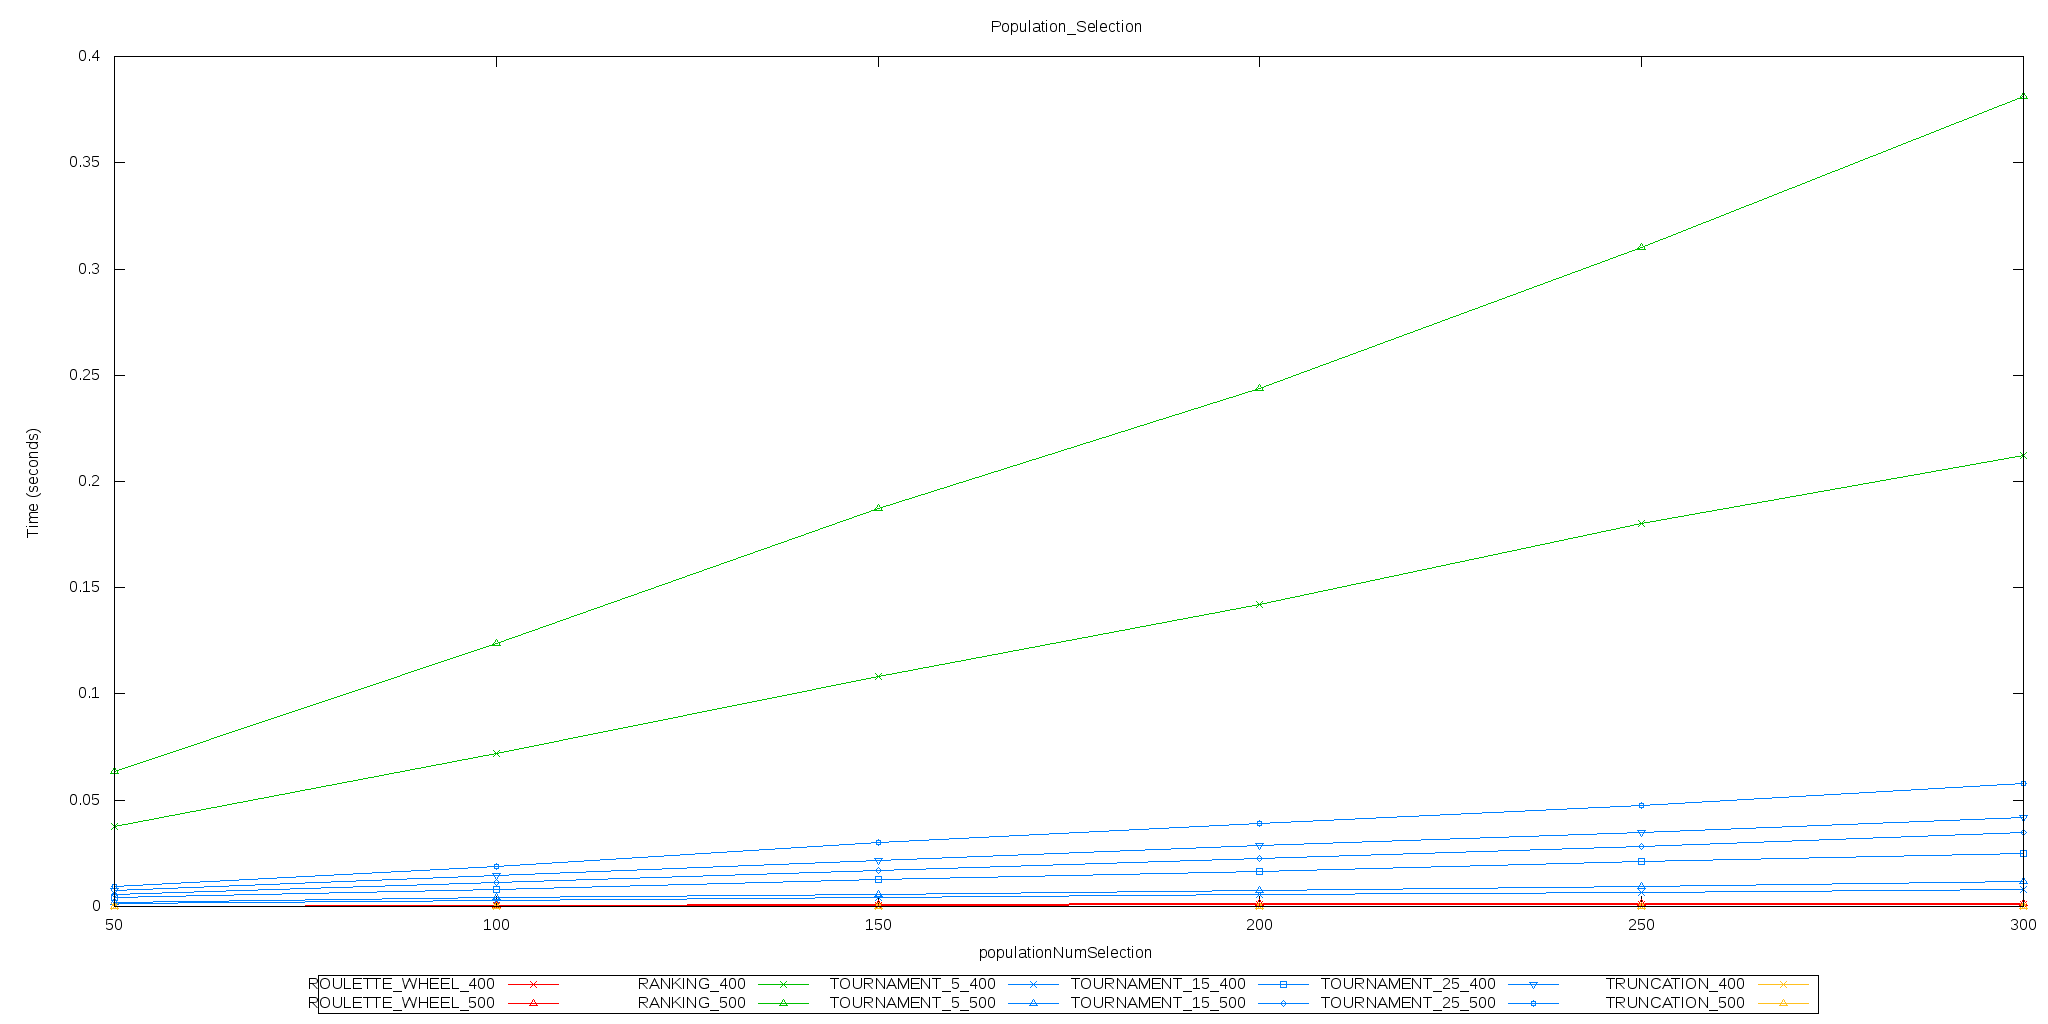
\includegraphics[width=\textwidth]{./img/Population_Selection.png}
\caption{\label{rendGenSelect}Rendimiento de los distintos operadores de selección en función del número de individuos a seleccionar. Cada operador se prueba con tamaños totales de población 400 y 500. Además, para la selección por torneo se muestran los resultados con varios tamaños de torneo.}
\end{figure}
\newpage
\paragraph{Cruza}
\label{sec-6-1-2-2}


figura \ref{rendGenCruza}

Como muestra la figura \ref{rendGenCruza} el nivel de cruza más costoso es el propio peso, el más barato es el nivel de capa completa y los niveles de neurona tienen rendimientos intermedios y parecidos independientemente de cómo se interprete qué pesos pertenecen a una neurona (si los pesos de entrada a la neurona o los pesos de salida de la misma).

En general, parece que el cruce uniforme es más costoso que el multi-punto y también es más costoso cuanto más se acerque al 50\% la probabilidad de coger el peso de un padre o de otro. El algoritmo multi-punto, sin embargo, no presenta diferencias de rendimiento significativas para 1 punto o 6 puntos de corte.

\begin{figure}[htb]
\centering
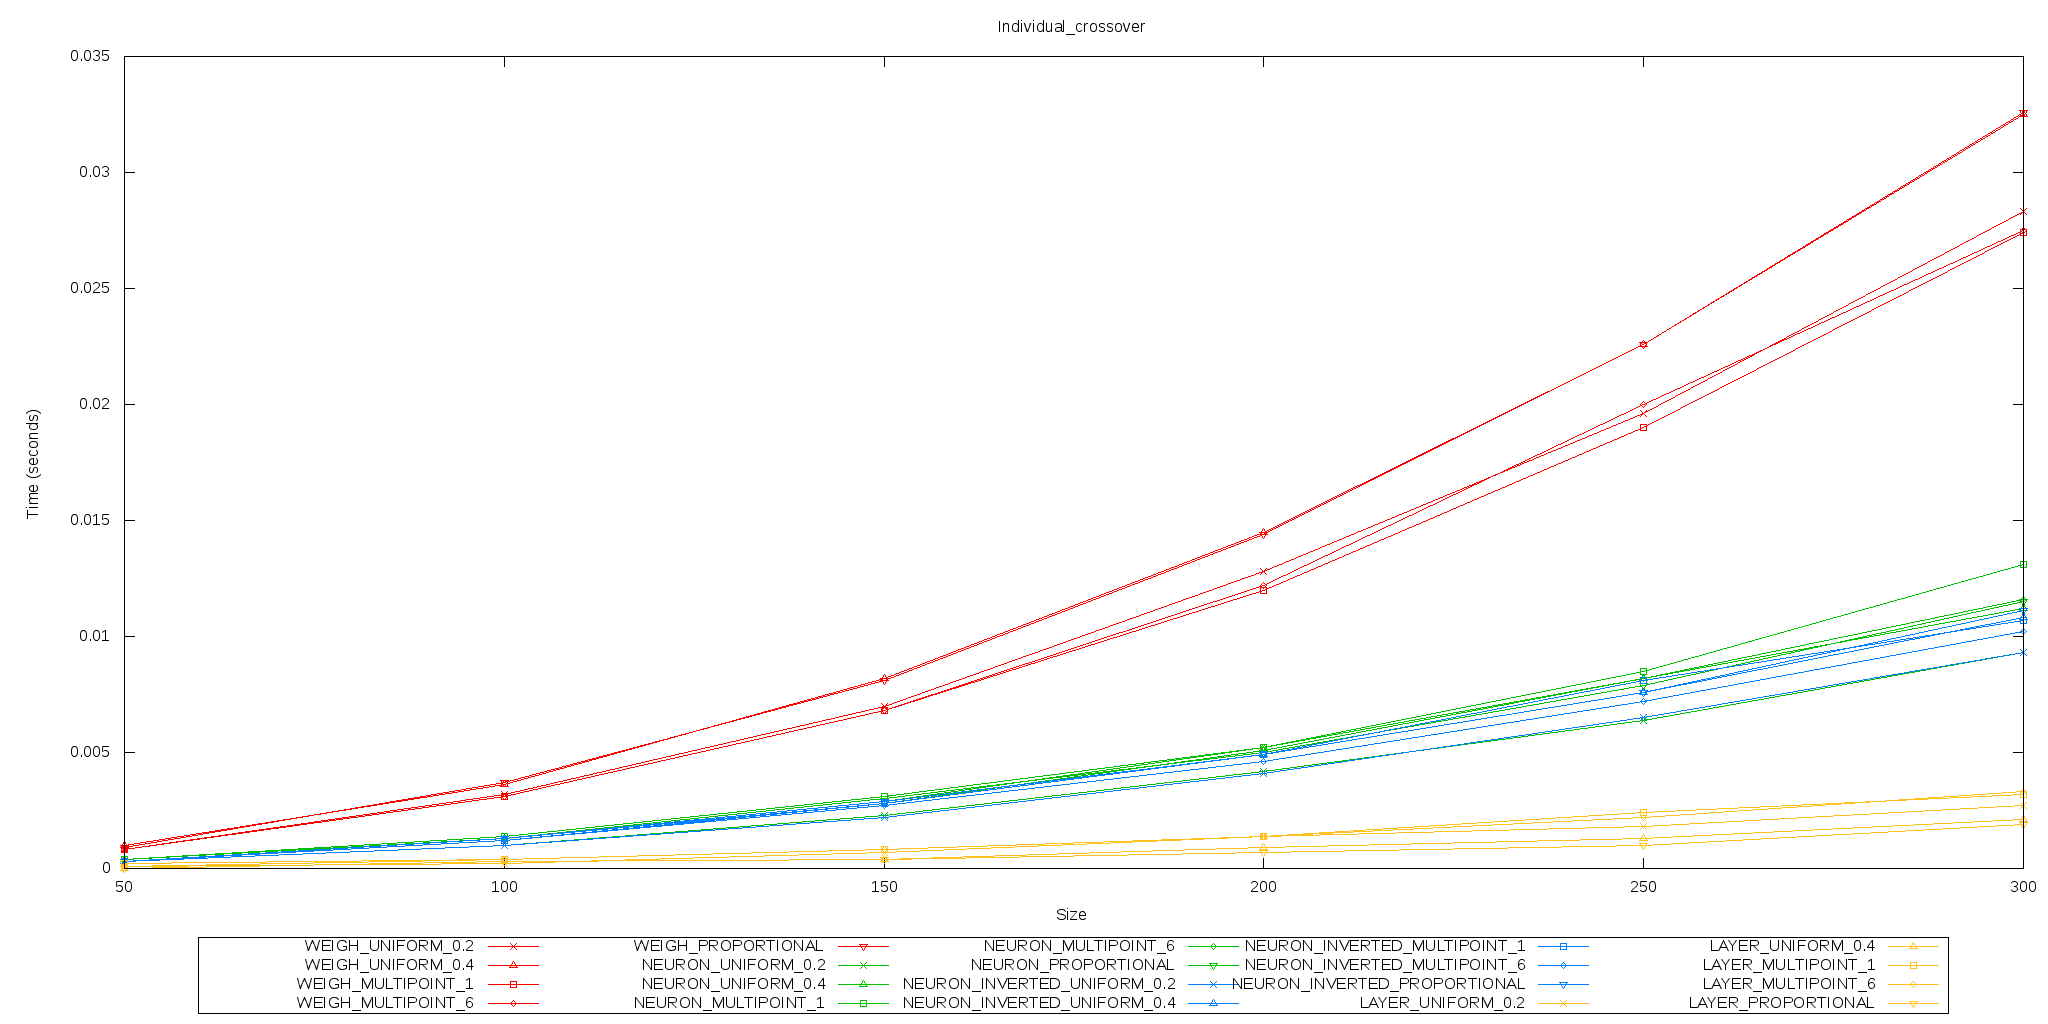
\includegraphics[width=\textwidth]{./img/Individual_crossover.png}
\caption{\label{rendGenCruza}Rendimiento de los distintos operadores genéticos de cruza en función del tamaño de las capas de neuronas internas.}
\end{figure}
\newpage
\paragraph{Mutación}
\label{sec-6-1-2-3}


Según la figura \ref{rendGenMutation}, ambos tipos de mutación son más costosos cuánto mayor es la probabilidad, tal y cómo era de esperar, pues más mutaciones son más escrituras. Además, la mutación probabilística es en general más costosa que la mutación determinística (un número constante de mutaciones por individuo) salvo cuando la probabilidad es muy grande (muchas mutaciones por individuo). Aunque la interfaz determinística es más rápida, también se hace más lenta comprativamente cuanto mayor es la probabilidad. La explicación es que la opción probabilística tiene un coste fijo elevado (un número aleatorio por gen) mientras que en la determinística el coste sube con el número de mutaciones (varios números aleatorios por cada mutación a realizar).

\begin{figure}[htb]
\centering
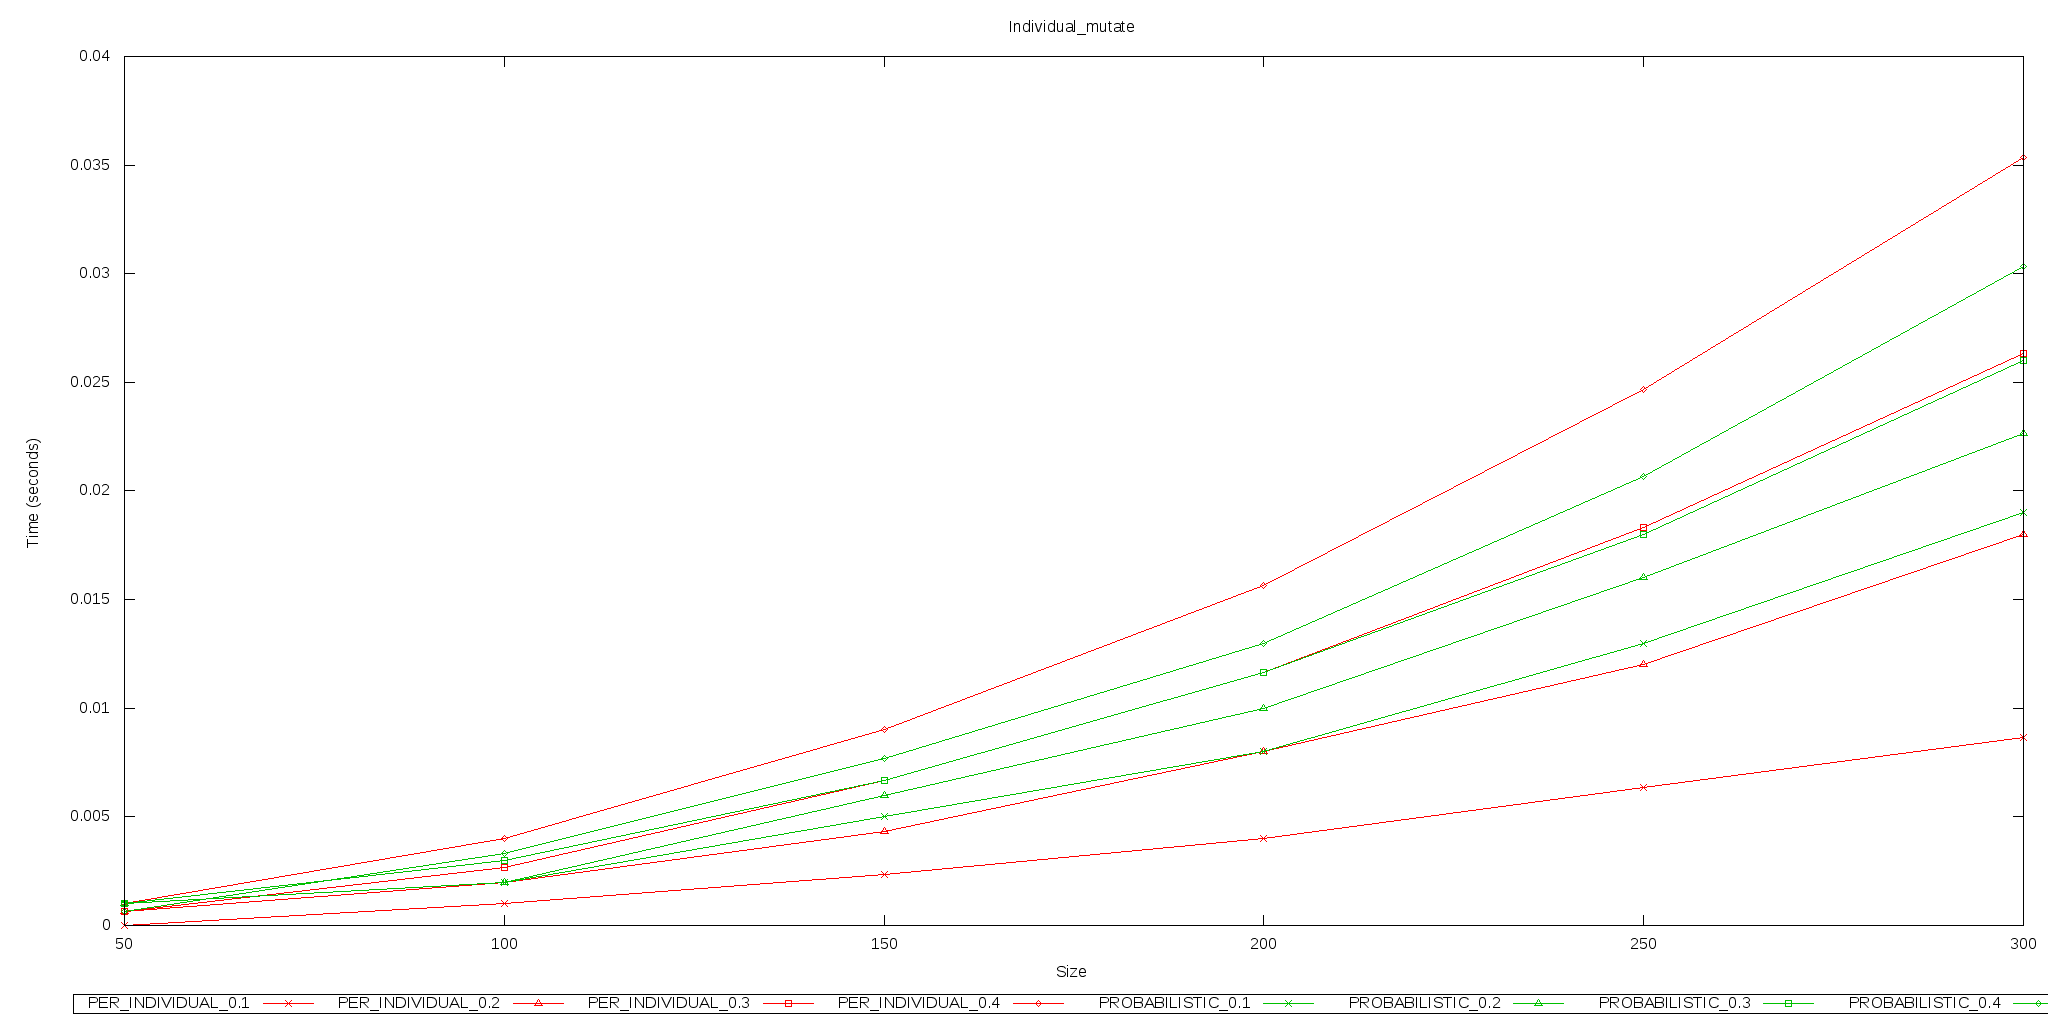
\includegraphics[width=\textwidth]{./img/Individual_mutate.png}
\caption{\label{rendGenMutation}Rendimiento de los distintos operadores genéticos de mutación para diferentes probabilidades. Para el operador no probabilístico, se ha calculado el número de mutaciones por individuo multiplicando la probabilidad por el número de genes (pesos y umbrales), para poder compararlo en igualdad con el operador probabilístico en cuanto al número de escrituras en los pesos.}
\end{figure}
\newpage
\paragraph{Olvido}
\label{sec-6-1-2-4}


El nuevo operador de olvido/reset presenta otra vez unos resultados similares a los de la mutación y se pueden extraer conclusiones semejantes como muestra la figura \ref{rendGenOlvido}.

\begin{figure}[htb]
\centering
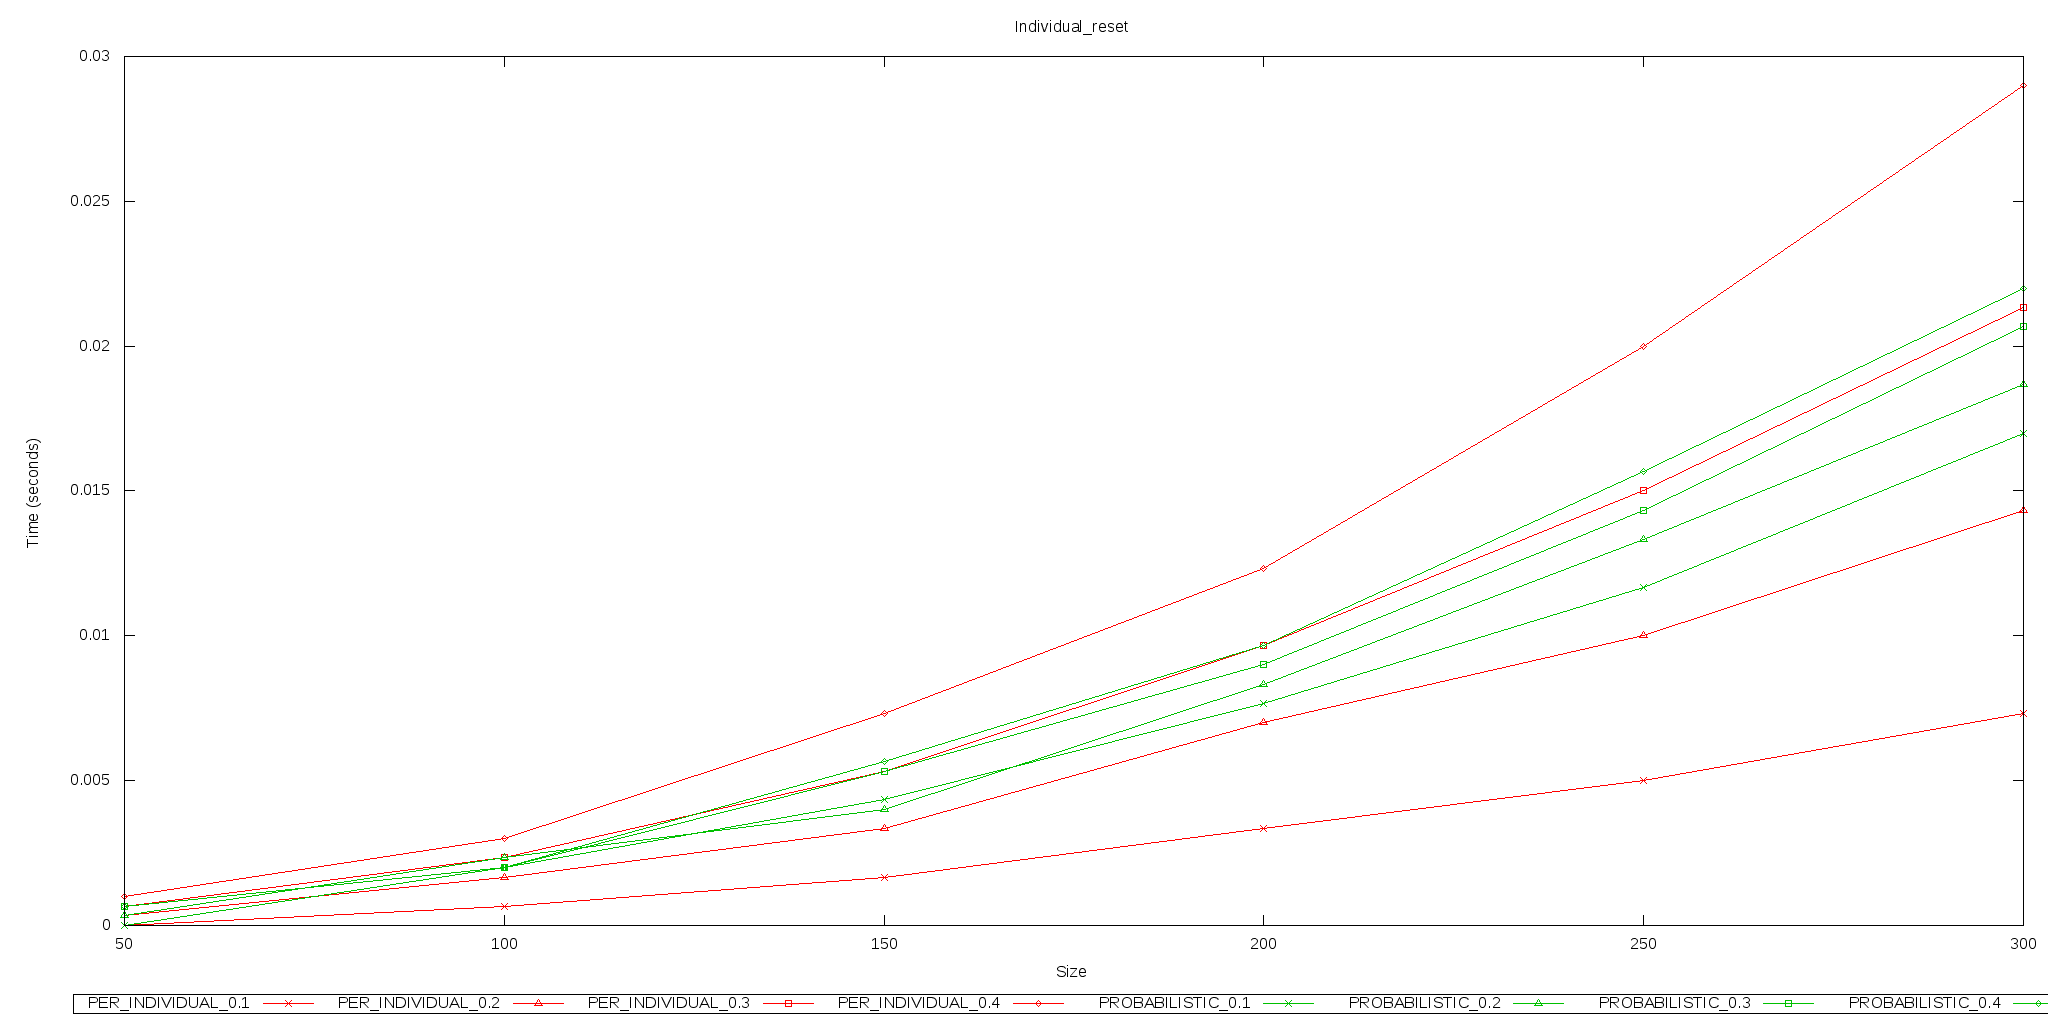
\includegraphics[width=\textwidth]{./img/Individual_reset.png}
\caption{\label{rendGenOlvido}Rendimiento de los distintas interfaces del nuevo operador genético de olvido para diferentes probabilidades. Para el operador no probabilístico, se ha calculado el número de mutaciones por individuo multiplicando la probabilidad por el número de genes (pesos y umbrales), para poder compararlo en igualdad con el operador probabilístico en cuanto al número de escrituras en los pesos.}
\end{figure}
\newpage
\subsection{Aprendizaje}
\label{sec-6-2}

  \label{aprendizaje}

En esta sección se muestran resultados de aprendizaje en términos del mejor fitness de la población en cada generación.
\subsubsection{Comparación entre distintas funciones de activación}
\label{sec-6-2-1}
\subsubsection{Comparaci\'on entre redes discretas y lineales}
\label{sec-6-2-2}

   \label{aprendDiscretLineales}

A continuación compararemos los posibles efectos beneficiosos o perjudiciales al aprendizaje que se pueden obtener a partir de renunciar a las funciones derivables en favor de neuronas de tipo BIT (salida 0 ó 1)  o SIGN (salida -1 ó 1) y de pesos discretos y más reducidos (1 Byte en lugar de los 4 bytes de un float).
\paragraph{OR}
\label{sec-6-2-2-1}


\begin{figure}[htb]
\centering
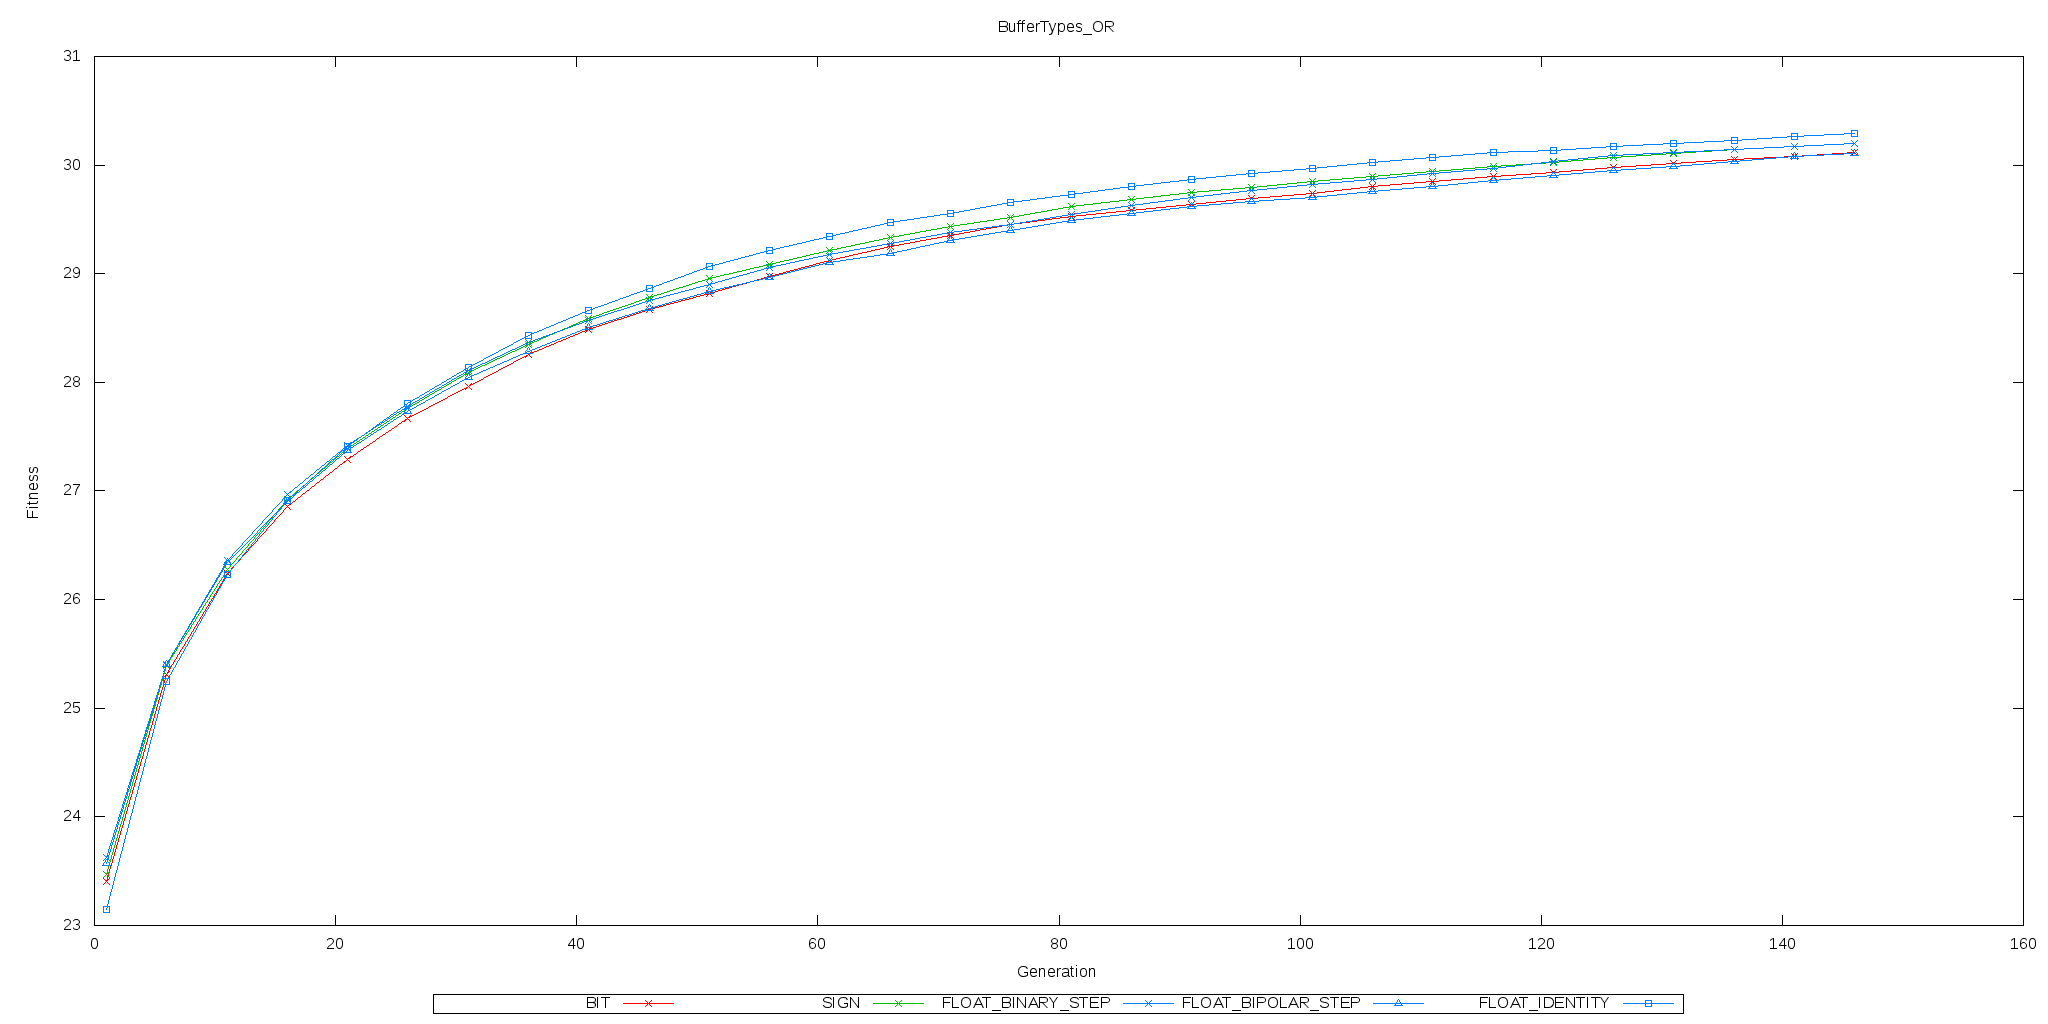
\includegraphics[width=\textwidth]{./img/BufferTypes_OR.png}
\caption{\label{aprenDiscretOr}Aprendizaje de la tarea lógica Or con los distintos tipos de neuronas (Binarias, bipolares y lineales).}
\end{figure}

\newpage
\paragraph{AND}
\label{sec-6-2-2-2}


\begin{figure}[htb]
\centering
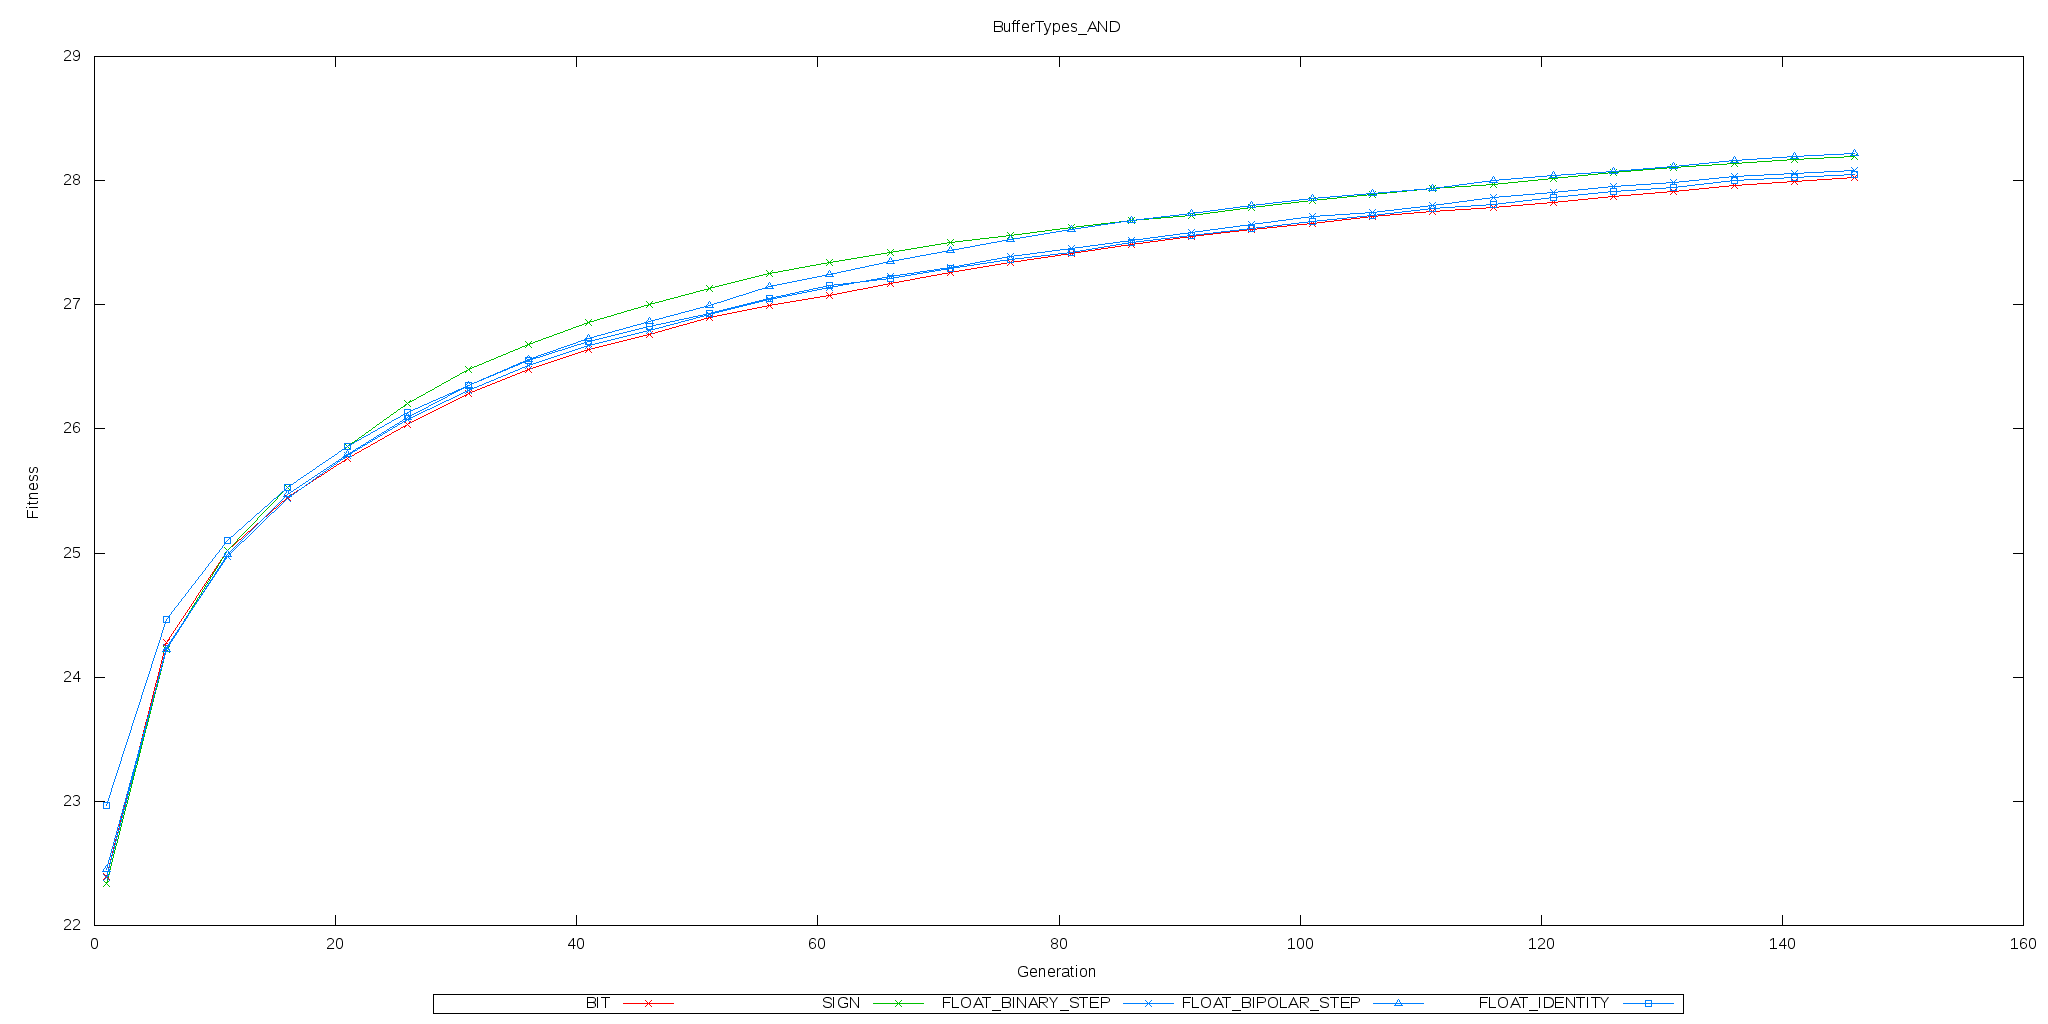
\includegraphics[width=\textwidth]{./img/BufferTypes_AND.png}
\caption{\label{aprenDiscretAnd}Aprendizaje de la tarea lógica And con los distintos tipos de neuronas (Binarias, bipolares y lineales).}
\end{figure}

\newpage
\paragraph{XOR}
\label{sec-6-2-2-3}


\begin{figure}[htb]
\centering
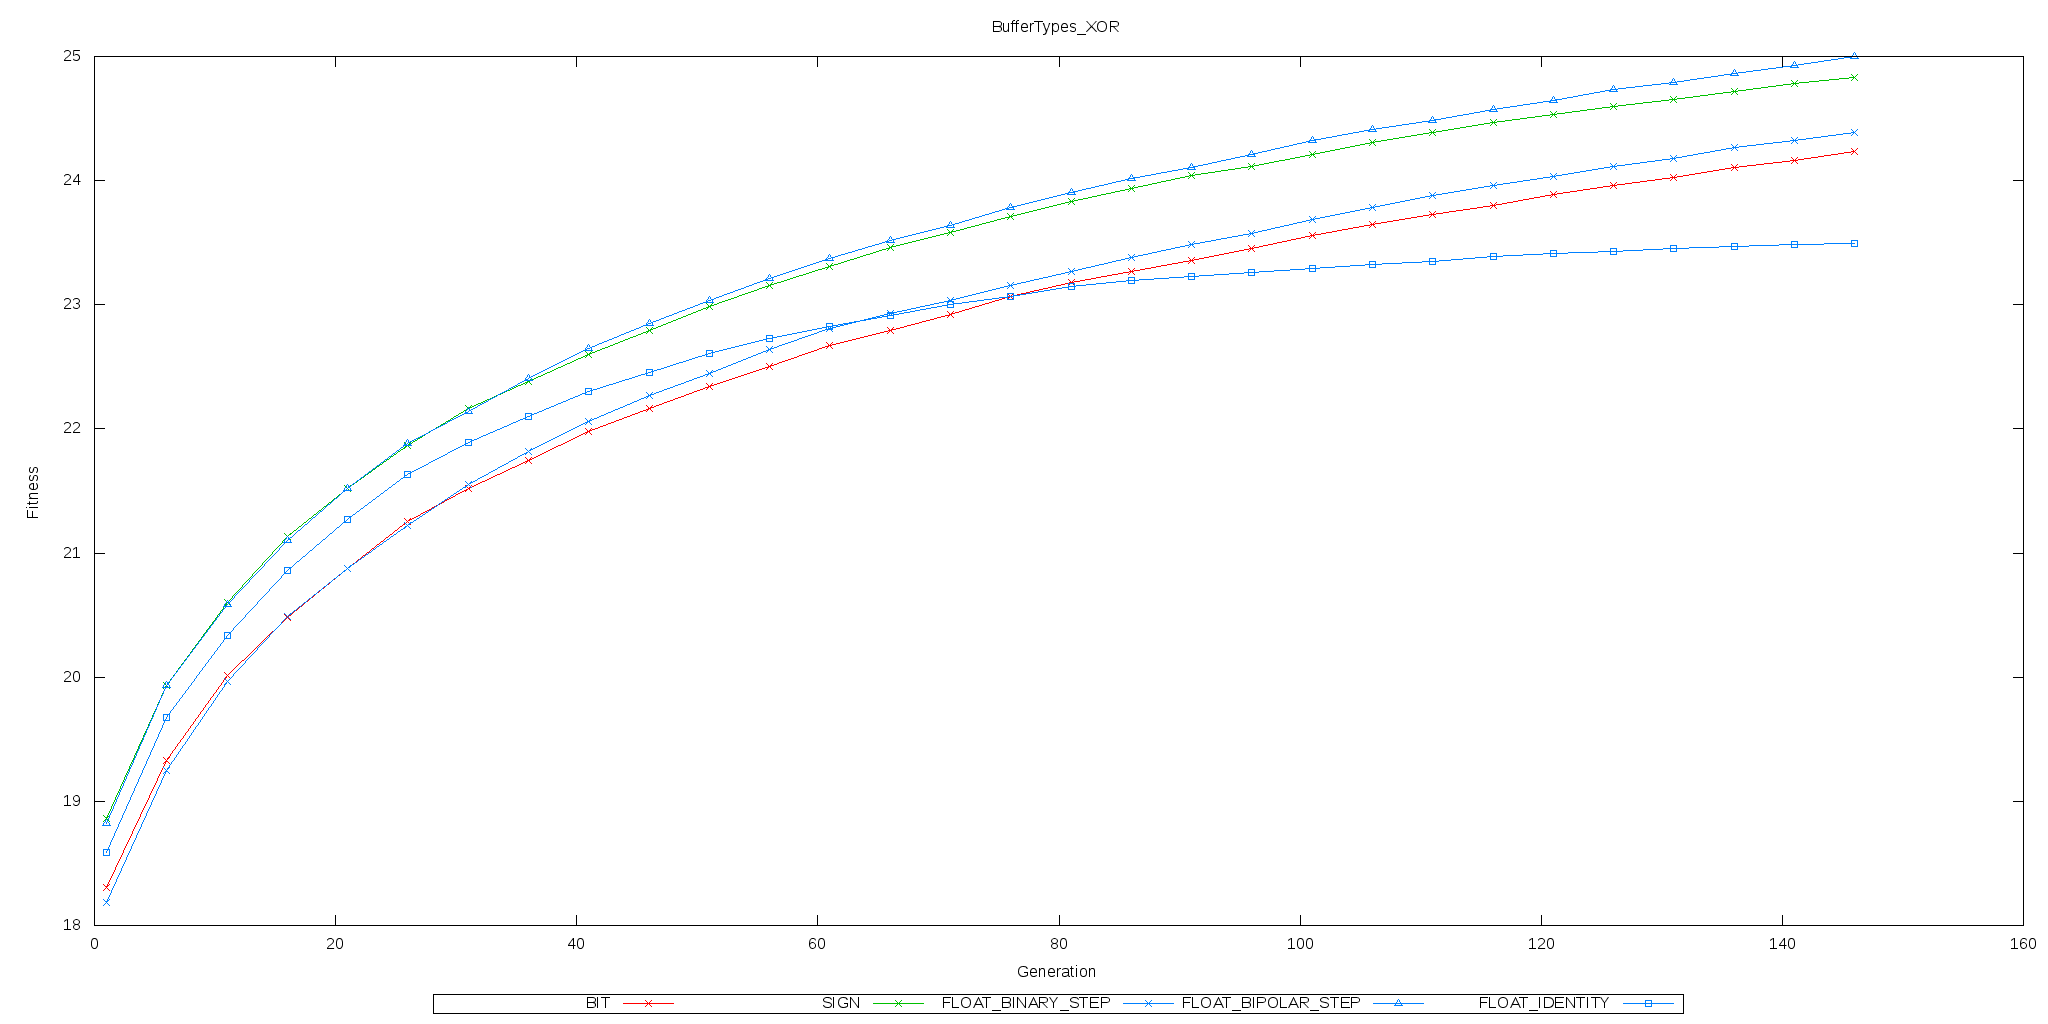
\includegraphics[width=\textwidth]{./img/BufferTypes_XOR.png}
\caption{\label{aprenDiscretXor}Aprendizaje de la tarea lógica Xor con los distintos tipos de neuronas (Binarias, bipolares y lineales).}
\end{figure}

\newpage
\paragraph{Reversi}
\label{sec-6-2-2-4}


\begin{figure}[htb]
\centering
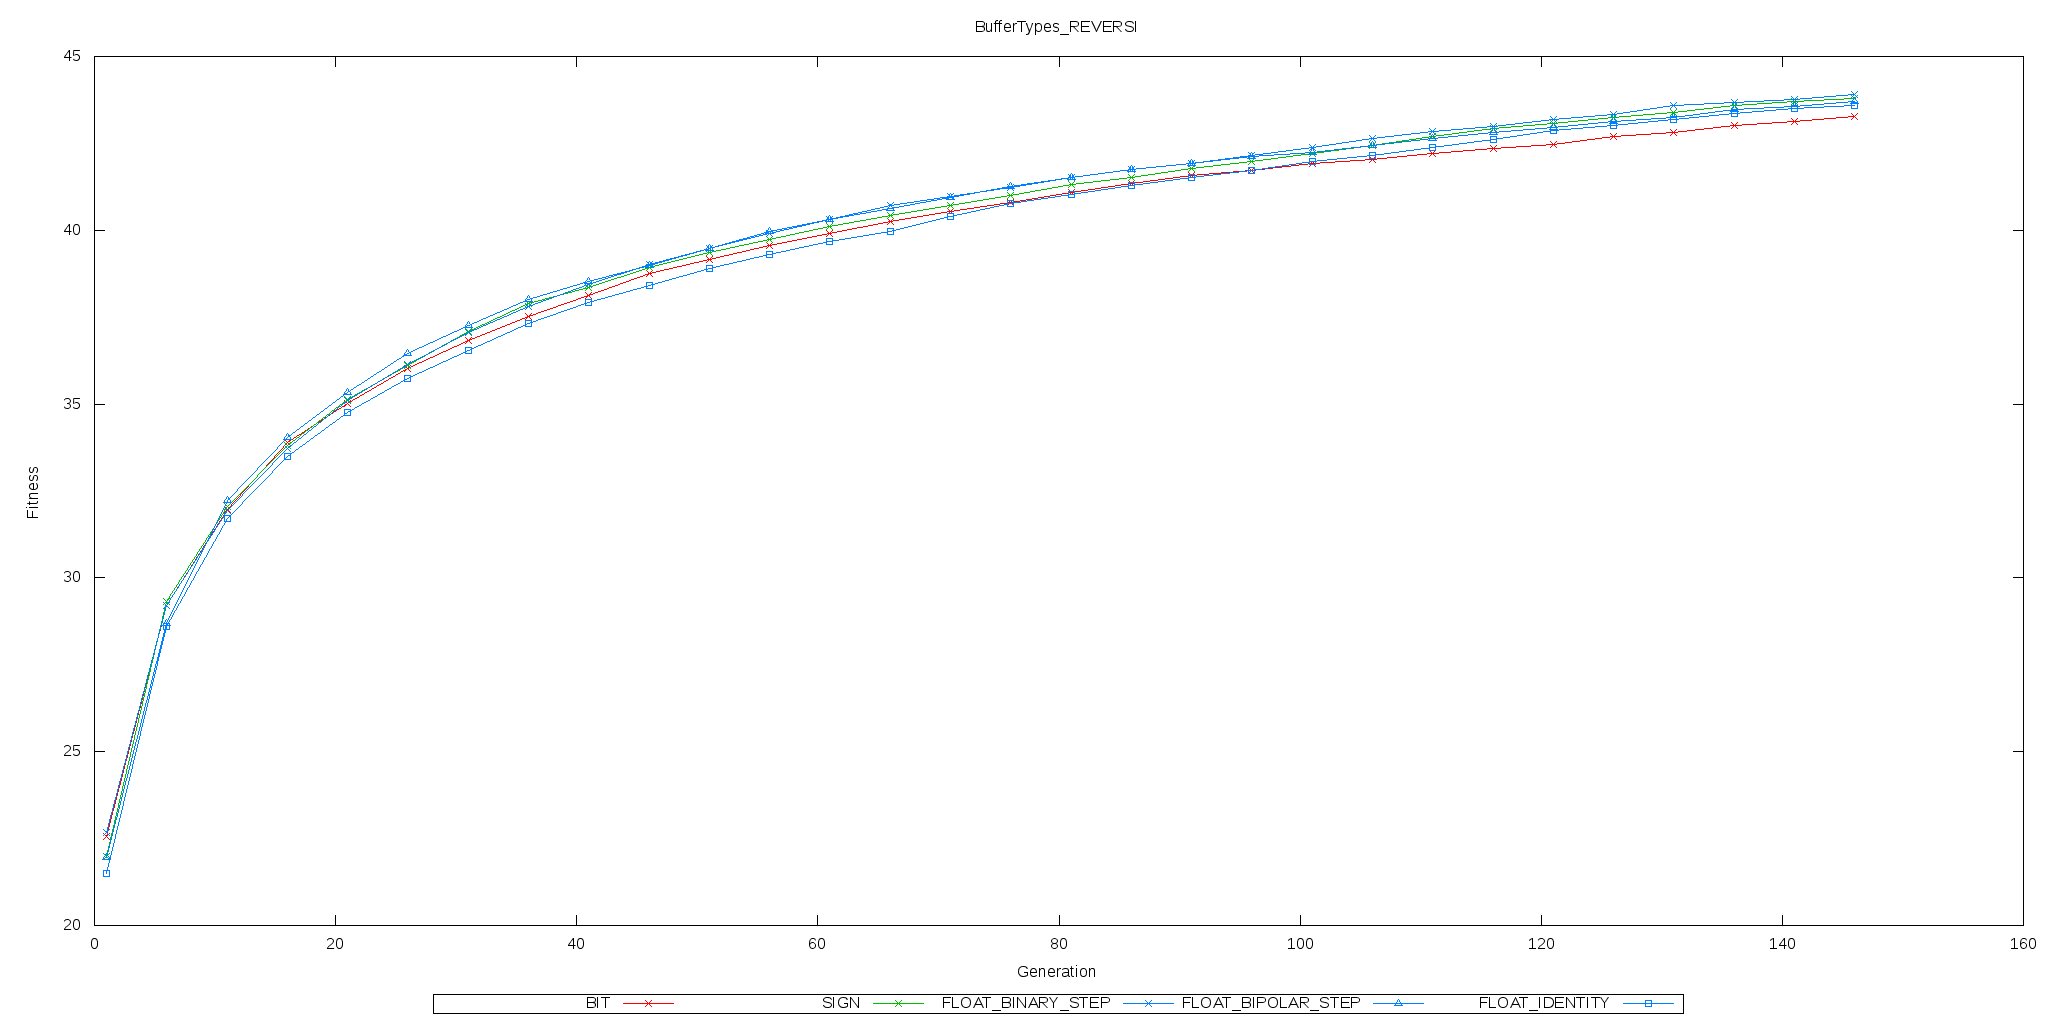
\includegraphics[width=\textwidth]{./img/BufferTypes_REVERSI.png}
\caption{\label{aprenDiscretReversi}Aprendizaje de la tarea Reversi con los distintos tipos de neuronas (Binarias, bipolares y lineales).}
\end{figure}

\newpage
\subsubsection{Comparaci\'on de operadores gen\'eticos}
\label{sec-6-2-3}

   \label{}
\paragraph{Selección}
\label{sec-6-2-3-1}


\newpage
\paragraph{Cruza}
\label{sec-6-2-3-2}


\newpage
\paragraph{Mutación}
\label{sec-6-2-3-3}


\newpage
\paragraph{Operador de olvido}
\label{sec-6-2-3-4}


\newpage
\subsubsection{Comparación de distintos tamaños de población número de individuos conservados por generación}
\label{sec-6-2-4}


\newpage
\section{Conclusiones}
\label{sec-7}

  \label{conclusiones}

\newpage

\cleardoublepage\phantomsection
\addcontentsline{toc}{chapter}{\bibname}
\begin{thebibliography}{9}
 
%\cite[texto]{etiqueta}

%
% No he puesto todas las referencias que tenía porque tenía demasiadas y no tengo muy claro qué tengo que hacer cuando unos se citan a otros. 
% Por ejemplo, he dejado muchas citas que Bertona hacía de otros y no sé si eso es correcto. Yao en una sóla frase referencia a muchísima gente y no sé muy bien qué debería hacer.
%Desde luego, he aprendido que la bibliografía es mejor prepararla sobre la marcha que al toda final.
%

  \bibitem{Yao99} \textsc{Xin Yao}: \emph{Evolving Artificial Neural Networks}. School of Computer Science, The University of Birmingham (1999).

  \bibitem{GomezMiikkulainen2003} \textsc{Faustino J. G\'omez y Risto Miikkulainen}: \emph{Robust Non-Linear Control through Neuroevolution}. Deparment of Computer Science, The University of Texas (2003).

  \bibitem{Bertona2005} \textsc{Luis Federico Bertona}: \emph{Entrenamiento de redes neuronales basado en algoritmos evolutivos}. Faculad de ingenier\'ia, Universidad de Buenos Aires (2005).


\end{thebibliography}

\end{document}
